%-------------------------------- Configurações --------------------------------

\documentclass[
  a4paper,         % Tamanho do papel: A4
	abntfigtabnum,
  noindentfirst,
	normaltoc,
	pnumplain,
	notimes
	% capchap,
]{abnt}

%\usepackage[bjarne]{fncychap}
\usepackage[utf8]{inputenc}
\usepackage[brazil]{babel}
\usepackage{url}
\usepackage{array}
\usepackage{graphicx}
\usepackage{subfigure}
\usepackage{enumerate}
\usepackage{multirow}
\usepackage{booktabs}
\usepackage[pdfborder={0 0 0}]{hyperref} % http://www.tug.org/applications/hyperref/manual.html
\usepackage[alf]{abntcite}
\usepackage{listings} % http://www.atscire.de/index.php?nav=products/listings2 http://linorg.usp.br/CTAN/macros/latex/contrib/listings/listings.pdf
\usepackage{textcomp}
\usepackage[usenames,dvipsnames]{xcolor} % http://en.wikibooks.org/wiki/LaTeX/Colors
\usepackage[portugues,algoruled,longend]{algorithm2e}
\usepackage{mathtools, mhsetup} % fórmulas matemáticas
\usepackage[usenames,dvipsnames]{pstricks} % gerar os gráficos
\usepackage{epsfig} % gerar os gráficos
\usepackage{float} % dependência do H para posição
\usepackage[all,cmtip]{xy}

\urlstyle{same} % http://en.wikibooks.org/wiki/LaTeX/Hyperlinks#Customization

%-------------------------------- Highligthing ---------------------------------

\lstset{
    language=C,
    basicstyle=\footnotesize\ttfamily,
    columns=flexible,
    numberbychapter=false,
    showstringspaces=false,
    tabsize=2,
    xleftmargin=17pt,
    framexleftmargin=17pt,
    framexrightmargin=5pt,
    framexbottommargin=4pt,
    numbers=left,
    numberstyle=\scriptsize\ttfamily\color{Gray},
    emphstyle=\color{OrangeRed},
    commentstyle=\color{Gray}\textit,
    stringstyle=\textit,
    keywordstyle=\textbf,
    morekeywords={@self, @caller, @const, @local},
    % emph={[2]Funcionalidade, Como},
    % emphstyle=[2]\color{MidnightBlue},
}

\usepackage{caption}
\DeclareCaptionFont{white}{\color{white}\footnotesize\bfseries}
\DeclareCaptionFormat{listing}{\colorbox{BrickRed}{\parbox{\textwidth}{#1#2#3}}}
\captionsetup[lstlisting]{format=listing,labelfont=white,textfont=white}

% Renomear listing e listings -> código e códigos
%\renewcommand*\lstlistingname{Código}
%\renewcommand*\lstlistlistingname{Lista de Códigos}

%--------------------------------- Informações ---------------------------------
\newcommand{\meutitulo}{A Programação Linear na classificação de dados em padrões}
\begin{document}

\titulo{\meutitulo}
\autor{Renata Gomes Cordeiro}
\instituicao{Universidade Estadual do Norte Fluminense Darcy Ribeiro}
\orientador[Tutor: ]{Fermín Alfredo Tang Montané.}
\comentario{Monografia apresentada ao Curso de Graduação em Ciência da
Computação da Universidade Estadual do Norte Fluminense Darcy Ribeiro como
requisito para obtenção do título de Bacharel em Ciência da Computação, sob
orientação do Profº. Fermín Alfredo Tang Montané.}
\local{Campos dos Goytacazes/RJ}
\data{2013}

\graphicspath{{graficos/}}
\capa
\folhaderosto

\sumario

\chapter{Introdução}

\section{Considerações Iniciais}
A programação linear é uma das disciplinas que compõem a programação matemática e constitui um dos pilares da pesquisa operacional. As aplicações da programação linear estão presentes em diversos setores, tais como nas indústrias, nos transportes, na saúde, na educação, na administração pública. etc.  Além disso, a resolução de problemas de programação linear (PPL) é requerida em outras disciplinas da programação matemática como programação inteira e programação não-linear, onde é comum a resolução de vários PPL de forma repetida.

O método simplex proposto por \citeonline{Dan} é um dos métodos mais conhecidos e eficientes para resolver problemas de programação linear. Trata-se de um dos poucos algoritmos que foi implantado comercialmente há mais de 40 anos. Atualmente, está presente em softwares comerciais tais como CPLEX e LINGO. Um método alternativo, teoricamente superior ao método simplex, é o método dos pontos interiores, proposto por \citeonline{Karmarkar}. Na prática, tanto o método simplex, quanto o método dos pontos interiores competem até hoje.  
(FALAR O QUE É O SIMPLEX REVISADO)
O presente trabalho, por opção, é focado especificamente no método simplex revisado. Busca-se o desenvolvimento de um aplicativo capaz de resolver problemas de programação linear utilizando o método simplex revisado. Acredita-se que a importância desse trabalho se deve ao intuito de explorar o conhecimento a respeito do método, e acima disso o desenvolvimento de uma ferramenta gratuita que proporcione ao usuário uma interface intuitiva e de fácil entendimento.

\section{Objetivos e justificativas}
O objetivo do presente trabalho é o estudo da utilização da programação linear, mais especificamente o método simplex, no reconhecimento de expressões faciais. 

Através desse estudo deve ser possível verificar a eficiência da programação linear nesse tipo de aplicação da computação gráfica. Além disso, devem ser realizadas duas comparações do resultado final obtido, do ponto de vista computacional: a utilização da programação linear e outro método mais comumente utilizado na computação gráfica; e a utilização de uma biblioteca desenvolvida e uma implementação do modelo de progra,ação linear utlizando o softwrae Cplex.

A programação linear possui aplicações em diversas áreas, como: indústria, produção, saúde e computação gráfica. Porém é um método mais comumente utilizado na engenharia de produção em problemas como: alocação de recursos e planejamento de produção. O presente trabalho justifica-se pelo fato de querer abordar uma aplicação prática dentro da computação, mais especificamente na computação gráfica, onde a aplicação da programação linear não é tão explorada quanto na engenharia de produção.

\section{Metodologia}
Para o cumprimento do obejtivo final, o trabalho é composto por algumas etapas:

\begin{itemize} 
\item O estudo do método simplex revisado, suas características, vantagens do ponto de vista computacional e suas variantes.
\item O desenvolvimento da biblioteca para resolução de problemas de programação linear
\item A implementação do modelo do problema de programação linear no software Cplex
\item Aplicação da biblioteca e da implementação feita no Cplex em alguma aplicação de computação gráfica para reconhecimento de expressões faciais.
\end{itemize}

Para a reralização desta última etapa, espera-se, através de pesquisas encontrar uma aplicação pronta que realize o reconhecimento de expressões faciais que deverá ser utilizada. Porém ao invés de realizar o processamento utilizando o método já incorporado à aplicação, o método simplex será utilizado. Caso não seja encontrada uma aplicação de reconhecimento de expressão facial, que torne viável a substituição do método utilizado, uma ferramenta de forneça essa funcionalidade será desenvolvida.

\section{Estrutura do trabalho} (COLOCAR A ESTRUTURA COMPLETA DA  MONOGRAFIA)
O presente trabalho apresenta a seguinte estrutura: o capítulo 2 apresenta uma descrição do problema geral de programação linear, os principais métodos de solução, algumas aplicações práticas e as ferramentas computacionais disponíveis. 

\chapter{Referencial teórico}
Este capítulo apresenta um revisão teórica sobre as principais metodologias utilizadas nesse trabalho: programação linear, métodos de classificação e métodos de validação. Também é apresentada uma revisão de trabalhos sobre classificação de dados.  

\section{A programação linear}
Na pesquisa operacional, a programação linear é uma das técnicas mais utilizadas para resolver problemas de otimização. Os problemas de programação linear geralmente buscam a distribuição eficiente de recursos limitados para atender um determinado objetivo, por isso suas aplicações estão presentes em diversas áreas como computação, administração, indústria e transporte \cite{Engecom}.

Um problema de programação linear é expresso através de um modelo composto por equações e inequações lineares. Esse tipo de problema busca a distribuição eficiente de recursos com restrições para alcançar um objetivo, em geral, maximizar lucros ou minimizar custos. Em um problema de programação linear esse objetivo é expresso através de uma equação linear denominada função objetivo. Para a formulação do problema, é necessário também definir os recursos necessários e em que proporção são requeridos. Essas informações são expressas em equações ou inequações lineares, uma para cada recurso. Esse conjunto de equações ou inequações é denominado restrições do modelo \cite{Engecom}.

\section{Descrição do problema de programação linear}
O modelo de um problema de programação linear é apresentado em uma das formas a seguir:
\noindent
\underline{\bf Modelo 1}
\begin{eqnarray}
    Max\ z = c^{T}x \label{eq:obj1}
\\s.a.\left\{\begin{matrix}
Ax\leq b\\*x\geq 0
\end{matrix}\right.\label{eq:rest1}
\end{eqnarray}
\\
\noindent
\underline{\bf Modelo 2}
\begin{eqnarray}
Min\ z = c^{T}x \label{eq:obj2}
\\*s.a.\left\{\begin{matrix}
Ax\geq  b\\*x\geq 0 
\end{matrix}\right. \label{eq:rest2}
\end{eqnarray}

Nos Modelos 1 e 2 as equações \ref{eq:obj1} e \ref{eq:obj2} representam as funções objetivo e as inequações \ref{eq:rest1} e \ref{eq:rest2} representam as restrições.
Onde, 
\begin{itemize}
\item \textbf {$x$} é o vetor com as variáveis do modelo
\item \textbf {$c$} é o vetor de coeficientes da função objetivo
\item \textbf {$z$} é o valor da função objetivo
\item \textbf {$A$} é a matriz com as constantes das restrições
\item \textbf {$b$} é o vetor com os valores limites das restrições
\end{itemize}

Sendo que c, A e b são dados conhecidos.

A seguir é apresentado um exemplo de aplicação da programação linear no contexto da otimização da produção. Uma empresa, que fabrica vários produtos, deseja maximizar o lucro na venda de dois desses produtos.
A produção é feita em três setores diferentes e está sujeita a restrições de tempo disponível para a produção em cada setor.
O problema pode ser representado pelo seguinte modelo de programação linear com duas variáveis\cite{Hillier}.

\begin{eqnarray}
Maximize\ z=3x_{1}+5x_{2}\label{eq2:eq1}\\ 
Sujeito\ a \nonumber \\ 
1x_{1}\leq 4 \label{eq2:eq2} \\  
2x_{2}\leq 12 \label{eq2:eq3} \\ 
3x_{1}+2x_{2}\leq 18 \label{eq2:eq4}\\ 
x_{1}\geq 0, x_{2}\geq 0 \label{eq2:eq5}
\end{eqnarray}

Onde, 
\begin{itemize}
\item \textbf {$x_{1}$} representa a quantidade do produto 1 produzido em uma semana.
\item \textbf {$x_{2}$} representa a quantidade do produto 2 produzido em uma semana.
\item \textbf {$z$} representa o lucro total por semana de produção desses dois produtos (em milhões de dólares), sendo o lucro do produto 1 de 3 milhões e o do produto 2 de 5 milhões.
\end{itemize}

E as restrições representam as restrições de tempo de cada setor que compõe o processo de produção.
\begin{itemize}
\item A equação \ref{eq2:eq2} garante que, durante o processo de produção, cada produto 1 necessita de 1 hora no setor 1, e o setor só tem disponível 4 horas por semana.
\item A equação \ref{eq2:eq3} garante que, durante o processo de produção, cada produto 2 necessita de 2 horas no setor 2, e o setor só tem disponível 12 horas por semana.
\item A equação \ref{eq2:eq4} garante que, durante o processo de produção, cada produto 1 necessita de 3 horas no setor 3, e cada produto 2 necessita de 2 horas no setor 3, e o setor só tem disponível 18 horas por semana.
\item A equação \ref{eq2:eq5} garante que, os dois produtos devem ser produzidos.
\end{itemize}

Um problema de programação linear com até três variáveis pode ser representado graficamente utilizando três eixos cartesianos. Os problemas com duas variáveis podem ainda ser facilmente resolvidos por meio da representação gráfica \cite{Passos}. 

A seguir, o problema exemplo é apresentado graficamente. Apesar de, na prática os modelos de programação linear possuírem um número de variáveis muito maior que dois ou três, a visualização gráfica do modelo, mesmo que simples, contribui para o entendimento dos métodos de resolução apresentados no capítulo a seguir.
\begin{center}
	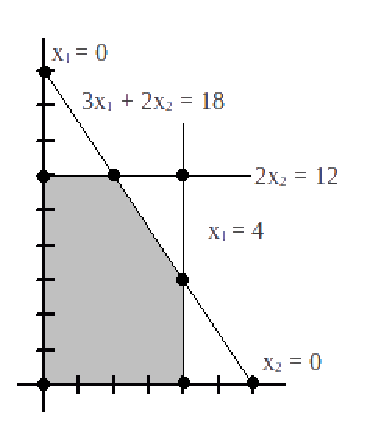
\includegraphics[scale=1.0]{graficos/simplex_graf}
	\captionof{figure}{Representação gráfica do modelo de programação linear de duas variáveis}
	\label{img:simplex_grafico}
\end{center}


Onde cada reta representa uma restrição do modelo, e a área cinza representa a região viável, ou seja, nessa área estão contidas os valores viáveis de $x_{1}$ e $x_{2}$ para a maximização do lucro.

Os métodos para resolução de problemas de programação linear buscam esses valores de $x_{1}$ e $x_{2}$  para a determinação da solução ótima.

\section{Aplicações utilizando programação linear}
Um problema de programação linear, como já dito anteriormente, busca um resultado ótimo sujeito a restrições, com utilização em diversas áreas.

A programação linear se aplica na área da saúde, como demonstrado por \citeonline{Alterovitz-saude} em seu trabalho. Em um determinado tipo de tratamento de câncer são inseridos cateteres na área afetada para introduzir o medicamento necessário, porém o medicamento acaba afetando células saudáveis além das cancerígenas. Como os problemas de programação linear podem ser resolvidos como problemas determinísticos e com solução exata, \citeonline{Alterovitz-saude} propõe a formulação de um problema de otimização para determinar o tempo de permanência dos cateteres, minimizando os desvios em relação a quantidade da dose necessitada pelo paciente através da minimização de custos atribuídos. Nos testes realizados, foi obtida uma melhoria nos desvios em relação a quantidade da dose necessitada pelo paciente mas clinicamente os resultados obtidos não mostraram uma vantagem significativa em relação ao método atualmente utilizado.

Em \citeonline{Moreira2003Saude} modelos de programação linear foram desenvolvidos para duas aplicações relacionadas a área da saúde. Em um dos modelos busca-se a formulação de uma dieta com custo mínimo, considerando as restrições alimentares e os nutrientes essenciais em uma dieta. Um segundo modelo visa analisar intervenções médicas que buscam maximizar os anos de vida de pacientes considerando uma população, como restrições são utilizados os custos e o número de visitas médicas. Para a resolução dos modelos foi utilizado o método simplex. O autor considerou a programação linear como um instrumento útil na tomada de decisões na área da saúde, considerando a importância da substituição de métodos tradicionais baseados no bom senso e tentativa de acerto por métodos com soluções otimizadas.

Nos trabalhos de \citeonline{Alterovitz-saude} e \citeonline{Moreira2003Saude} foi exemplificado como a programação pode ser útil e importante na área da saúde. No primeiro trabalho apesar de não demonstrar uma melhoria no resultado geral, foi comprovada a equivalência dos resultados com o método probabilístico atualmente utilizado. Em \citeonline{Moreira2003Saude} apesar dos dados utilizados serem reduzidos e uma dieta real possuir mais restrições que as propostas no trabalho, o autor demonstrou a aplicabilidade da programação linear em duas situações da área da saúde.

Em \citeonline{Possami2011Logistica} a programação linear foi utilizada na resolução de um problema abrangendo o transporte, o processamento e a estocagem de fumo, buscando como objetivo a minimização dos custos. O modelo proposto foi composto por 650 variáveis e 150 restrições. A partir do resultado obtido foi possível determinar parâmetros desde o transporte da matéria bruta, estocagem até a venda do produto.

Dentre as aplicações mais conhecidas da programação linear, encontram-se os problemas de planejamento de produção e controle de estoque, assuntos relacionados a engenharia de produção, como no trabalho de \citeonline{Possami2011Logistica}. A partir desse trabalho tem-se o exemplo de como os resultados extraídos de um modelo de programação linear podem ser determinantes no sucesso de um processo de produção.

Em seu trabalho \citeonline{Krukoski2010Economia} propõe a utilização da programação linear na economia. Considerando que os investimentos em ações estão cada vez mais acessíveis para pequenos investidores, o autor propõe um modelo de programação linear na determinação de uma operação de compra ou venda que maximize o lucro e baseando-se também nos riscos. Os resultados obtidos em sua maioria foram positivos e lucrativos, apesar de, de acordo com o autor, algumas operações obtidas nos resultados serem pouco aplicáveis se comparadas às atitudes rotineiras dos investidores.

No trabalho proposto por \cite{Krukoski2010Economia} foi apresentada uma aplicação que pode auxiliar na tomada de decisões na área da economia. Os bons resultados mostram que a programação linear, como método determinístico, pode ser empregada mesmo em problemas que estão mais relacionados a métodos probabilísticos, como é o caso dos investimentos em ações.

A programação linear além de estar presente, é fundamental em diversas áreas, tornando-se uma ferramenta de apoio a decisão e contribuindo para o sucesso de projetos nas áreas em que se aplica.

\section{Métodos de classificação}
Em problemas de classificação, dado um conjunto de dados dividido entre conjunto de treinamento e conjunto de teste, onde, no conjunto de treinamento cada subconjunto pertence a um entre \textit{n} padrões, o objetivo é que a partir de um dado do conjunto de teste o método de classificação retorne a qual dos \textit{n} padrões esse dado pertence. A seguir são apresentados alguns dos métodos de classificação mais citados na literatura. 

\subsection{\it Support Vector Machines}
\textit{Support Vector Machines} (SVM) ou Máquinas de vetores de suporte têm a capacidade de gerar classificadores na etapa de treinamento e de classificar os dados na etapa de teste de acordo com os classificadores gerados. Considerando um problema de classificação com dois padrões, uma SVM irá determinar um plano que separe os pontos desses dois padrões, de forma que a distância entre o hiperplano e os pontos seja a máxima possível. Os pontos de cada padrão utilizados como referência são denominados vetores de suporte.
No caso de conjuntos linearmente inseparáveis, é utilizada um função denominada Kernel. Essa função é responsável por elevar a dimensão espacial a fim de que os pontos se tornem linearmente separáveis. Portanto para a obtenção de um classificador utilizando SVM é necessária a escolha de uma função kernel e os parâmetros dessa função. Essa escolha influencia diretamente no desempenho do classificador\cite{Gunn98SVM}\cite{Reffson02SVM}.

No caso em que o número de padrões é maior que dois, duas abordagens podem ser utilizadas com as SVM \cite{Lorena03SVM}:
\begin{itemize}
\item{\textbf{Um contra todos:} }Nessa abordagem, para \textit{k} padrões são geradas \textit{k} SVM. Na criação das SVM, é gerado um hiperplano que separa 1 padrão dos \textit{k}-1 padrões. Na determinação do padrão de um dado x, o padrão é aquele que, entre as \textit{k} SVM obteve x do lado do hiperplano onde se encontrava o padrão separado dos demais.  
\item{\textbf{Todos contra um:} }Nessa abordagem os padrões são agrupados em pares e uma SVM é gerada para cada par. Um esquema de votação deve ser utilizado para determinar o padrão de uma instância, que deve ser analisada a partir de cada SVM e cada SVM retorna um padrão possível. O padrão que obtiver mais pontos da instância é a classe atribuída.
\end{itemize}

\subsection{\it Naive Bayes}
Na metodologia \textit{Naive Bayes} as características do dado a ser classificado são analisadas de forma independente. O vetor de características é formado pela número de vezes que cada característica ocorre no dado caracterizado. A probabilidade de uma instância pertencer a um determinado padrão é dada por uma probabilidade inicial, baseada na quantidade total de dados, e pelas probabilidades das ocorrências das características \cite{McCallum98Bayes} \\
\cite{Langley92Bayes}. %Essa abordagem é mais comumente utilizada na área de mineração de dados, onde dada uma palavra busca-se o melhor texto baseado na quantidade de vezes que a palavra aparece da palavra no textos utilizados no treinamento% \

\subsection{\textit{k}- nearest neighbor}
Nesse método a classificação é feita pela similaridade da instância a ser classificada com um dado ou vetor utilizado no treinamento, a classe do dado utilizado no treinamento é então atribuída a instância com padrão inicialmente desconhecido. As etapas desse método consistem em utilizar um parâmetro para medir a semelhança ou a distância do dado a ser classificado em relação a cada um dos dados utilizados no treinamento. Os \textit{k} vetores mais similares ou mais próximos são selecionados e entre o padrão mais frequente é atribuído ao dado inicialmente desconhecido. Apesar de ser considerado um método simples, sua dificuldade está em definir os parâmetros ou a métrica que definirá a semelhança ou distância entre os dados\cite{Chagas09KNN}.

\subsection{Redes Neurais Artificias}
Em seu trabalho  \citeonline{Morais2010RNA} define Redes Neurais Artificiais (RNA) como sistemas paralelos e distribuídos compostos por unidades de processamento simples (neurônios) interligadas por conexões, esses neurônios calculam determinadas funções matemáticas. Na fase de treinamento ou aprendizagem "um conjunto de exemplos é apresentado a rede que extrai automaticamente características necessárias para representar a informação fornecida" \cite{Morais2010RNA}.
Uma rede neural pode receber como entrada, na etapa de treinamento, um conjunto de vetores com seus respectivos padrões. Ao submeter como entrada um vetor com padrão desconhecido a rede neural deve classificar esse vetor. A vantagem desse método é que uma rede pode construir fronteiras não lineares entre padrões, o que pode ser muito vantajoso em problemas complexos de classificação. Existem vários modelos de redes neurais que possibilitam o reconhecimento de padrões, entre eles: Perceptron de Camada Simples, Perceptron de Múltiplas e Redes de Kohonen \cite{ZubenRNA2}.

\section{Aplicações em classificação de dados}
Em seu trabalho \citeonline{Reffson02SVM} busca o classificação de impressões digitais em 5 padrões. Esse tipo de classificação tem o propósito de gerenciar grandes bancos de dados de impressões digitais e acelerar o processo de identificação. Foi utilizado um banco contendo 4000 imagens igualmente distribuídas entre os cinco padrões. O autor dividiu o banco em dois grupos, utilizando um para treinamento e outro para teste. Após a extração das características das imagens, Máquinas de Vetores de Suporte foram utilizadas na classificação. Na abordagem todos contra um foi obtida uma média de precisão de 91,18\%, já na abordagem um contra todos a precisão na classificação das impressões foi de 90,43\%.

\citeonline{Chagas09KNN} apresentou uma técnica para a classificação de textos, uma atividade importante em aplicações como bibliotecas digitais e em outras que em geral buscam a organização de documentos disponíveis no formato digital. O autor propôs variações no método \textit{k near neighbor} a fim de  aprimorar a escolha dos textos, utilizados no treinamento, mais próximos ao texto que precisa ser classificado. Nos testes feitos com três coleções de textos, as médias de acertos na classificação obtidas foram acima de 90\% em duas coleções, e próxima a 70\% na terceira.

No trabalho de \citeonline{sbai2003RNALaranjas} uma rede neural artificial foi utilizada na classificação de laranjas através de imagens. Os autores consideraram que apesar da automação de muitos setores industriais, em um sistema de produção, as frutas consideradas boas, são selecionadas através de inspeção visual humana. A principal característica utilizada foi a cor, que pode classificar a fruta em cinco padrões. No trabalho ficou comprovada a aplicabilidade do método para o domínio proposto que era classificar as frutas de acordo com a cor.

\section{Métodos de validação da metodologia}
Uma metodologia de classificação pode ser verificado em relação a sua acurácia a partir de um conjunto de dados ou a sua performance em relação a outros métodos classificadores. Algumas técnicas utilizadas com esse intuito serão apresentadas a seguir. No presente trabalho a técnica Cross Validation é utilizada com o objetivo de verificar a acurácia, nesse caso, da metodologia utilizada na classificação de dados.

A seguir são apresentadas as três técnicas mais comumente encontradas na bibliografia com suas ventagens e desvantagens:

\subsection{\textit{Handout}}
Esse é um método simples, onde os dados são divididos em 2 grupos mutuamente exclusivos, sendo um grupo utilizado para treino e o outro para teste. Em geral 2/3 dos dados são utilizados no treinamento e 1/3 na etapa de testes. Os dois grupos devem conter dados suficientes de todos os padrões, nesse caso, suficientes para que o resultado final não seja comprometido pela falta de dados, de um determinado padrão, no grupo da etapa de treino e nem no grupo de testes. Apesar de ser um método de fácil implementação, a divisão entre conjunto de treinamento e teste deve ser bem estudada de forma que todos os padrões estejam bem representados nos dois grupos, por isso é um método recomendável quando o conjunto de dados possui um grande número de representações de cada padrão \cite{Kohavi95Cross} \cite{Baldisserotto05Validacao}.

\subsection {\textit{Cross Validation}}
Nesse método, o conjunto de dados também é dividido em conjunto de treinamento e de teste, porém esses dois grupos variam a cada rodada de teste. O tipo de \textit{cross validation} mais comumente utilizado é o \textit{k-fold cross validation}, onde os dados são divididos em k conjuntos mutuamente exclusivos e as etapas de treinamento e teste são realizadas k vezes, de forma que a cada rodada um conjunto diferente é utilizado como teste e os outros k-1 conjuntos são utilizados para treinamento. Esse método é recomendável quando o conjunto de dados não é tão grande, pois não existe uma  preocupação de quais dados separar para teste e quais separar para treinamento, já que ao final da execução do método todos o dados terão participado dos conjuntos de treinamento e teste \cite{Kohavi95Cross} \cite{Baldisserotto05Validacao}.

\subsection{\textit{Leave-one-out}}
Nessa técnica, do conjunto com o número total de dados n, são realizadas n rodadas de treinamento e teste, sendo que a cada rodada n-1 dados são utilizados para teste e o dados restantes são utilizados para treinamento. Pelas suas características, esse é um método recomendável para conjuntos de dados pequenos já que a quantidade de rodadas de treinamento e teste é igual a quantidade de dados o que o torna um método com alto custo computacional \cite{Kohavi95Cross} \cite{Baldisserotto05Validacao}.

\chapter{Métodos de Solução}
Entre os métodos mais utilizados para a resolução de problemas de programação linear destaca-se o método simplex  e o método de pontos interiores. 
Depois da apresentação do método simplex,outros métodos com diferentes abordagens foram propostos \cite{Todd}. Porém, dentre os métodos existentes apenas o método de pontos interiores é atualmente competitivo em relação ao método simplex \cite{Bixby}. 
A principal diferença entre esses dois métodos é que o método simplex busca a solução ótima em um dos vértices da região viável, enquanto o método de pontos interiores percorre o interior da região viável definindo um caminho até a solução ótima \cite{MaculanPI}. Além disso, uma outra diferença é que o simplex exige muitas iterações com cálculos simples, enquanto no método de pontos interiores poucas iterações são exigidas, porém com cálculos mais elaborados.
Apesar das vantagens do método de pontos interiores em relação ao método estudado neste trabalho, o método simplex possui melhor desempenho na resolução de problemas de pequeno e médio porte em relação ao método de pontos interiores.

\section{Método Simplex}
O método simplex é um dos algoritmos mais conhecidos para a resolução de problemas de programação linear. Surgiu há mais de 60 anos atrás e foi proposto por George Dantzig.  

É um método iterativo, e sua ideia principal consiste no fato de que a cada iteração uma nova solução é encontrada, sempre melhor que a anterior até o ponto em que a solução ótima é obtida. Outra característica do método é o fato de ser matricial, ou seja, os dados a serem calculados são armazenados em matrizes.  

Com a utilização do método, foi percebido que a cada iteração eram requeridos muitos cálculos sobre valores que nem sempre importavam para a iteração seguinte, fato que do ponto de vista computacional tornaria o método ineficiente. Esse método é chamado de método simplex padrão ou tabular. A partir desse fato foi desenvolvido o método simplex revisado visando a resolução de problemas de programação linear computacionalmente.

\subsection{Princípio básico do método}
A idéia do método simplex consiste em resolver repetidas vezes um sistema de equações lineares, e assim obter uma sucessão de soluções até encontrar a solução ótima. Ou seja, é um processo onde nos movemos de uma solução viável para outra sempre melhor ou pelo menos não pior.

Um problema de programação linear é sempre constituído de uma função objetivo e várias restrições. Geometricamente, essas restrições resultam em uma forma geométrica, no espaço n-dimensional sendo n o número de variáveis no modelo. E cada vértice dessa forma geométrica é considerado como uma possível solução, retomando o exemplo apresentado na seção 2.2.
\begin{center}
	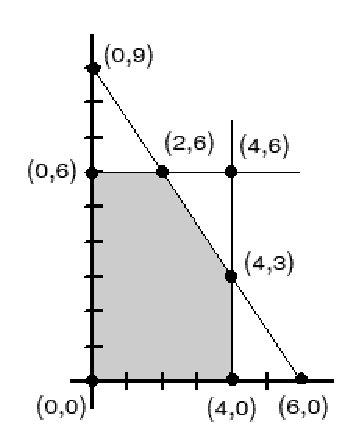
\includegraphics[scale=1.0]{graficos/graf_simplex_pontos}
	\captionof{figure}{Representação gráfica de um modelo de programação linear}
	\label{img:simplex_grafico_completo}
\end{center}

Nesse exemplo, de acordo com a representação geométrica do modelo, existem cinco possíveis soluções: ($x_{1}=0$ e $x_{2}=0$), ($x_{1}=0$ e $x_{2}=6$), ($x_{1}=2$ e $x_{2}=6$), ($x_{1}=4$ e $x_{2}=3$), ($x_{1}=4$ e $x_{2}=0$). Como o objetivo é maximizar, concluímos que a melhor solução é $x_{1}=2$ e  $x_{2}=6$, em que $z=36$. No método Simplex a cada iteração, antes da solução ótima ser obtida, é encontrada uma dessas possíveis soluções que se localizam nos vértices da forma geométrica.

\subsection{Descrição do Método Simplex Revisado}
O método simplex revisado surgiu como uma solução para evitar cálculos desnecessários. Esse método foi projetado para problemas a serem solucionados computacionalmente.

No simplex revisado, são armazenados na memória volátil apenas os dados realmente necessários. Além disso, os cálculos são realizados apenas sobre a coluna que é utilizada na iteração, o que evita cálculos com matrizes que poderiam acarretar uma imprecisão nos resultados.

Esse método mantém a característica do simplex, que é a troca entre a variável que entra na base e a que sai (as variáveis da base são as que contribuem para o valor da solução ótima), além de também exigir certo esforço computacional. Porém sua grande vantagem é a economia de tempo e espaço, que é garantida pelo modo como é desenvolvida a solução. 

Nesta seção são descritos os passos do algoritmo simplex revisado. O problema considerado é de maximização. A distinção entre matrizes, vetores e escalares foi feita da seguinte forma: letra maiúscula e negrito para matriz (\textbf{MATRIZ}); letra minúscula e negrito para vetor (\textbf{vetor}); letra em itálico para escalar (\textit{escalar}).

Para a resolução do problema através do método simplex revisado, é necessário que o problema de programação linear esteja na forma padrão. Dizemos que um problema de programação linear está na sua forma padrão quando estiver no seguinte formato:

$\\
Maximizar\ \mathbf{cx} \\
Sujeito\ a \\
\mathbf{Ax} = \mathbf{b} \\
\mathbf{x} \geq0$

ou

$\\
Minimizar\ \mathbf{cx} \\
Sujeito\ a \\
\mathbf{Ax} = \mathbf{b} \\
\mathbf{x} \geq0$

com $\mathbf{b}\geq0$.

Um problema de programação linear pode ser tranformado para a forma padrão acrescentando variáveis de folga, como no exemplo abaixo:

\begin{align*}
Maximize\ z=3x_{1}+5x_{2}\\ 
Sujeito\ a \\ 
1x_{1}\leq 4 \\  
2x_{2}\leq 12 \\ 
3x_{1}+2x_{2}\leq 18 \\ 
 x_{1}\geq 0, x_{2}\geq 0 \\
\end{align*}
Adicionando as variáveis de folga:
\begin{align*}
Maximize\ z=3x_{1}+5x_{2}\\ 
Sujeito\ a\\
1x_{1}+\ \ \ \ \ \ \ x_{3}\ \ \ \ \ \ \ \ \ \ \ = 4 \\  
2x_{2}+\ \ x_{4}\ \ \ \ = 12 \\ 
3x_{1}+2x_{2}+\ \ \ \ \ \ x_{5}= 18 \\ 
 x_{1}\geq 0, x_{2}\geq 0 \\
\end{align*}

A inserção das variáveis de folga formam uma matriz base na matriz de coeficientes das restrições, as variáveis correspondentes a essa matriz base são denomindas variáveis básicas. Inicialmente as variáveis básicas são as variáveis de folga.

O vetor $\mathbf{c}$, de coeficientes na função objetivo, é dividido em duas componentes: $\mathbf{c{_B}}$ e $\mathbf{c{_N}}$, coeficientes das variáveis básicas e não-básicas, respectivamente. Por analogia, o vetor $\mathbf{x}$, de incógnitas do problema, é subdividido em $\mathbf{x{_B}}$ e $\mathbf{x{_N}}$.  A matriz $\mathbf{A}$, de coeficientes das restrições, é dividida em duas submatrizes: $\mathbf{B}$ e $\mathbf{N}$, coeficientes das variáveis básicas e não-básicas, respectivamente. O vetor $\textbf{b}$ são os valores das restrições. Os passos do algoritmo são os seguintes.\\

\noindent
\framebox{
\begin{minipage}[l]{14,2cm}
\textbf{Passo 1}: Calcular o vetor multiplicador: \ \ $\mathbf{\lambda} \ =\ \mathbf{c{_B^t}B^{-1}}$
\\ \\
\textbf{Passo 2}: Escolher a variável que entra na base: $\mathbf{p}\ =\ \mathbf{c{_N}}-\mathbf{\lambda N}$

Se \ \ $\mathbf{p}\ =\ (\mathbf{c{_N}}-\mathbf{\lambda N})\leq 0$ \ \ PARAR. \\ A solução \ \ $\mathbf{x{_B}}$ \ \ já é a solução ótima. 

Se não, escolher uma coluna de $\mathbf{N}$, coluna $\mathbf{a{_k}}$, tal que $\mathit{p{_k}}\ =\ \mathit{c{_nk}}-\mathbf{\lambda a{_k}}> 0$

Um critério frequente é escolher a coluna $\mathbf{a{_k}}$ que resulte no maior valor de $\mathit{p{_k}}$.

Então, assumindo $\mathit{e} = \mathit{k}$, $\mathit{k}$ representa o índice da coluna, $\mathbf{a{_k}}$ representa a coluna de $\mathbf{A}$ candidata a entrar na base. 
\\ \\
\textbf{Passo 3}: Determinar a variável que sai da base: $\mathbf{y}=\mathbf{B^{-1}a{_k}}$

Se \ \ $\forall i\mathit{\frac{b{_i}}{y{_i}}}\leq 0$ \ \ PARAR, a solução é não-limitada. 

Senão, calcular:\ \ 
$\forall i\ \underset{\underset{y{_i}>0}{1\leq i\leq m}}{Min}\begin{Bmatrix}
\mathit{\frac{(x{_b}){_i}}{y{_i}}}
\end{Bmatrix}$ e guardar o índice correspondente a $s = i$. A variável $(x{_b}){_s}$ sai da base.
\\ \\
\textbf{Passo 4}: Criar a matriz $\mathbf{E}$.
$\mathbf{E}=(\mathbf{e{_1}},\mathbf{e{_2}},...,\mathbf{e{_s-1}},\mathbf{\gamma} , \mathbf{e{_s+1}},...,\mathbf{e{_m}})$

Onde, cada coluna da matriz é um vetor unitário com exceção da coluna $\mathit{s}$, que corresponde ao vetor $\mathbf{\gamma}$, calculado da seguinte maneira: \\
$\mathbf{\gamma^{t}}=\left( \mathit{\frac{-\mathbf{A} {_{1,e}}}{\mathbf{A} {_{s,e}}}}\ \mathit{\frac{-\mathbf{A} {_{2,e}}}{\mathbf{A} {_{s,e}}}}\ ...\ \mathit{\frac{-\mathbf{A} {_{s-1,e}}}{\mathbf{A} {_{s,e}}}}\ \mathit{\frac{1}{\mathbf{A} {_{s,e}}}\ \frac{-\mathbf{A} {_{s+1,e}}}{\mathbf{A} {_{s,e}}}}\ ...\ \mathit{\frac{-\mathbf{A} {_{m,e}}}{\mathbf{A} {_{s,e}}}} \right )$
\\ \\
\textbf{Passo 5}: Calcular nova matriz $\mathbf{B^{-1}}$: $\mathbf{B^{-1}} = \mathbf{EB^{-1}}$
\\ \\
\textbf{Passo 6}: Atualizar os vetores $\mathbf{c{_B}}$ e $\mathbf{x{_B}}$.
\end{minipage}
}


A seguir, o modelo de programação linear apresentado na seção 2.2 é resolvido através do método Simplex Revisado.

\noindent
\framebox{
\begin{minipage}[l]{14,2cm}
\begin{align*}
Maximize\ z=3x_{1}+5x_{2}\\ 
Sujeito\ a \\ 
1x_{1}\leq 4 \\  
2x_{2}\leq 12 \\ 
3x_{1}+2x_{2}\leq 18 \\ 
 x_{1}\geq 0, x_{2}\geq 0 \\
\end{align*}
Adicionando as variáveis de folga:
\begin{align*}
Maximize\ z=3x_{1}+5x_{2}\\ 
Sujeito\ a\\
1x_{1}+\ \ \ \ \ \ \ x_{3}\ \ \ \ \ \ \ \ \ \ \ = 4 \\  
2x_{2}+\ \ x_{4}\ \ \ \ = 12 \\ 
3x_{1}+2x_{2}+\ \ \ \ \ \ x_{5}= 18 \\ 
 x_{1}\geq 0, x_{2}= 0 \\
\end{align*}

	\textbf{Inicialização:}\\

 \ \ \ \ \ $\mathbf{x{_N}}=[x{_1}\ \ x{_2}]$ \ \ \ \ \ $\mathbf{x{_B}}=[x{_3}\ \ x{_4}\ \ x{_5}]$
 \ \ \ \ \ $\mathbf{B}=\begin{bmatrix}
1 & 0 & 0 \\
0 & 1 & 0 \\
0 & 0 & 1
\end{bmatrix} = \mathbf{B^{-1}}$
\\ $\mathbf{x{_B}}\mathbf{B}=\mathbf{b} \Rightarrow \mathbf{x{_B}}=\mathbf{B^{-1}}\mathbf{b}\Rightarrow\mathbf{x{_B}}=\begin{bmatrix}
x{_3} \\
x{_4} \\
x{_5} 
\end{bmatrix} = \begin{bmatrix}
1 & 0 & 0 \\
0 & 1 & 0 \\
0 & 0 & 1
\end{bmatrix}\begin{bmatrix}
4 \\
12 \\
18 
\end{bmatrix} = \begin{bmatrix}
4 \\
12 \\
18 
\end{bmatrix}$ \\$\mathbf{c{_B}}=[0\ \ 0\ \ 0]$
\ \ \ \ \ $z = \mathbf{c{_B}}\mathbf{x{_B}} = [0\ \ 0\ \ 0]\begin{bmatrix}
4 \\
12 \\
18 
\end{bmatrix} = 0$
 \ \ \ \ \ $\mathbf{c{_N}}=[3\ \ 5]$ \ \ \ \ \ $\mathbf{c{_B}}=[0\ \ 0\ \ 0]$ \ \ \ \ \ $\mathbf{A}=[\ \mathbf{N}\ |\ \mathbf{B}\ ]=\left [ \left.\begin{matrix}
1 & 0 \\
0 & 2 \\
3 & 2 
\end{matrix}\right|
\begin{matrix}
1 & 0 & 0 \\
0 & 1 & 0 \\
0 & 0 & 1
\end{matrix} \right ]$ \ \ \ \ \ 
\end{minipage}
}

\noindent
\framebox{
\begin{minipage}[l]{14,2cm}
\textbf{Iteração 1}
\\ \\
\textbf{Passo 1:} Calcular o vetor multiplicador
\\$\mathbf{\lambda} \ =\ \mathbf{c{_B^t}B^{-1}}$\\
$\mathbf{\lambda} \ =\begin{bmatrix}
1 & 0 & 0 \\
0 & 1 & 0 \\
0 & 0 & 1
\end{bmatrix}[0\ \ 0\ \ 0]=[0\ \ 0\ \ 0]$
\\ \\
\textbf{Passo 2:} Escolher a variável que entra na base
$\mathbf{p}\ =\ \mathbf{c{_N}}-\mathbf{\lambda N}$\\
$\mathbf{p}\ =\ [3\ \ 5]-[0\ \ 0\ \ 0]\begin{bmatrix}
1 & 0 \\
0 & 2 \\
3 & 2 
\end{bmatrix}=[3\ \ 5]$
\\$k=2$ a variável $(x_{N})_{k}$ entra na base, $(x_{N})_{k} = x_{2}$ .
\\ \\
\textbf{Passo 3:}Determinar a variável que sai da base
$\mathbf{y}=\mathbf{B^{-1}a{_k}}$\\
$\mathbf{y}=\begin{bmatrix}
1 & 0 & 0 \\
0 & 1 & 0 \\
0 & 0 & 1
\end{bmatrix}\begin{bmatrix}
0 \\
0 \\
2
\end{bmatrix}=\begin{bmatrix}
0 \\
0 \\
2
\end{bmatrix}$

$Min\begin{Bmatrix}
\frac{4}{0},\frac{12}{2},\frac{18}{2}
\end{Bmatrix} = \frac{12}{2}$\\
$s=2$ a variável $(x_{B})_{s}$ sai da base, $(x_{B})_{s}=x_{4}$ 
\\ \\
\textbf{Passo 4:} Criar a matriz $\mathbf{E}$.
\\$\mathbf{E}=\begin{bmatrix}
1 & 0 & 1\\
1 & \frac{1}{2} & 1\\
1 & -1 & 1
\end{bmatrix}$
\\ \\
\textbf{Passo 5:} Calcular nova matriz $\mathbf{B^{-1}}$ 
\\$\mathbf{B^{-1}} = \mathbf{EB^{-1}}$
\\$\mathbf{B^{-1}} = \begin{bmatrix}
1 & 0 & 1\\
1 & \frac{1}{2} & 1\\
1 & -1 & 1
\end{bmatrix}\begin{bmatrix}
1 & 0 & 0 \\
0 & 1 & 0 \\
0 & 0 & 1
\end{bmatrix}=\begin{bmatrix}
1 & 0 & 0 \\
0 & \frac{1}{2} & 0 \\
0 & -1 & 1
\end{bmatrix}$
\\ \\
\textbf{Passo 6:} Atualizar os vetores $\mathbf{c{_B}}$ e $\mathbf{x{_B}}$.
\\$\mathbf{c{_B}}=[0\ \ 5\ \ 0]$
 \ \ \ \ \ 
$\mathbf{x{_B}}=\begin{bmatrix}
x{_3} \\
x{_2} \\
x{_5} 
\end{bmatrix} = \begin{bmatrix}
1 & 0 & 0 \\
0 & \frac{1}{2} & 0 \\
0 & -1 & 1
\end{bmatrix}\begin{bmatrix}
4 \\
6 \\
6 
\end{bmatrix} = \begin{bmatrix}
4 \\
6 \\
6 
\end{bmatrix}$
 \ \ \ \ \ $z = [0\ \ 5\ \ 0]\begin{bmatrix}
4 \\
6 \\
6 
\end{bmatrix} = 30$
\end{minipage}
}

\noindent
\framebox{
\begin{minipage}[l]{14,2cm}
\textbf{Iteração 2}
\\ \\
\textbf{Passo 1:} Calcular o vetor multiplicador
\\$\mathbf{\lambda} \ =\ \mathbf{c{_B^t}B^{-1}}$\\
$\mathbf{\lambda} \ =\begin{bmatrix}
1 & 0 & 0 \\
0 & \frac{1}{2} & 0 \\
0 & -1 & 1
\end{bmatrix}[0\ \ 5\ \ 0]=[0\ \ \frac{5}{2}\ \ 0]$
\\ \\
\textbf{Passo 2:} Escolher a variável que entra na base
$\mathbf{p}\ =\ \mathbf{c{_N}}-\mathbf{\lambda N}$\\
$\mathbf{p}\ =\ [3\ \ 0]-[0\ \ \frac{5}{2}\ \ 0]\begin{bmatrix}
1 & 0 \\
0 & 1 \\
3 & 0 
\end{bmatrix}=[3\ \ -\frac{5}{2}]$
$k=1$ a variável $(x_{N})_{k}$ entra na base, $(x_{N})_{k} = x_{1}$.
\\ \\
\textbf{Passo 3:}Determinar a variável que sai da base
$\mathbf{y}=\mathbf{B^{-1}a{_k}}$\\
$\mathbf{y}=\begin{bmatrix}
1 & 0 & 0 \\
0 & \frac{1}{2} & 0 \\
0 & -1 & 1
\end{bmatrix}\begin{bmatrix}
1 \\
0 \\
3
\end{bmatrix}=\begin{bmatrix}
1 \\
0 \\
3
\end{bmatrix}$

$Min\begin{Bmatrix}
\frac{4}{1},\frac{6}{0},\frac{6}{3}
\end{Bmatrix} = \frac{6}{3} = 2$\\
$s=3$ a variável $(x_{B})_{s}$ sai da base, $x_{B})_{s} = x_{5}$
\\ \\
\textbf{Passo 4:} Criar a matriz $\mathbf{E}$.
\\$\mathbf{E}=\begin{bmatrix}
1 & 1 & -\frac{1}{3}\\
1 & 1 & 0\\
1 & 1 & \frac{1}{3}
\end{bmatrix}$
\\ \\
\textbf{Passo 5:} Calcular nova matriz $\mathbf{B^{-1}}$ 
\\$\mathbf{B^{-1}} = \mathbf{EB^{-1}}$
\\$\mathbf{B^{-1}} = \begin{bmatrix}
1 & 1 & -\frac{1}{3}\\
1 & 1 & 0\\
1 & 1 & \frac{1}{3}
\end{bmatrix}\begin{bmatrix}
1 & 0 & 0 \\
0 & \frac{1}{2} & 0 \\
0 & -1 & 1
\end{bmatrix}=\begin{bmatrix}
1 & \frac{1}{3} & -\frac{1}{3} \\
0 & \frac{1}{2} & 0 \\
0 & -\frac{1}{3} & \frac{1}{3}
\end{bmatrix}$
\\ \\
\textbf{Passo 6:} Atualizar os vetores $\mathbf{c{_B}}$ e $\mathbf{x{_B}}$.
\\$\mathbf{c{_B}}=[0\ \ 5\ \ 3]$
 \ \ \ \ \ $\mathbf{x{_B}}=[x{_3}\ \ x{_2}\ \ x{_1}]$
\\$\begin{bmatrix}
x{_3} \\
x{_2} \\
x{_1} 
\end{bmatrix} = \begin{bmatrix}
1 & 1 & -\frac{1}{3}\\
1 & 1 & 0\\
1 & 1 & \frac{1}{3}
\end{bmatrix}\begin{bmatrix}
4 \\
12 \\
18 
\end{bmatrix} = \begin{bmatrix}
2 \\
6 \\
2 
\end{bmatrix}$
 \ \ \ \ \ $z = [0\ \ 5\ \ 3]\begin{bmatrix}
2 \\
6 \\
2 
\end{bmatrix} = 36$
\end{minipage}
}

\noindent
\framebox{
\begin{minipage}[l]{14,2cm}
\textbf{Iteração 3}
\\ \\
\textbf{Passo 1:} Calcular o vetor multiplicador
\\$\mathbf{\lambda} \ =\ \mathbf{c{_B^t}B^{-1}}$\\ \\
\\$\mathbf{\lambda} \ =\begin{bmatrix}
1 & \frac{1}{3} & -\frac{1}{3} \\
0 & \frac{1}{2} & 0 \\
0 & -\frac{1}{3} & \frac{1}{3}
\end{bmatrix}[0\ \ 5\ \ 3]=[0\ \ \frac{3}{2}\ \ 1]$
\\ \\
\textbf{Passo 2:} Escolher a variável que entra na base
$\mathbf{p}\ =\ \mathbf{c{_N}}-\mathbf{\lambda N}$\\
$\mathbf{p}\ =\ [0\ \ 0]-[0\ \ \frac{3}{2}\ \ 1]\begin{bmatrix}
0 & 0 \\
0 & 1 \\
1 & 0 
\end{bmatrix}=[-1\ \ -\frac{3}{2}]$
\\Não há valor maior que 0, então chegamos a solução ótima.
$z=36$
\end{minipage}
}
\section{Método de Pontos Interiores}
Em 1984, Karmarkar revolucionou a área de programação linear com a publicação de um algoritmo de complexidade polinomial que apresentou bom desempenho quando aplicado a problemas práticos \cite{MaculanPI}. Essa publicação deu origem a um novo campo de pesquisa, chamado de método dos pontos interiores. 

O método de pontos interiores tem como principal característica realizar a busca por soluções no interior da região viável do problema, até encontrar a solução ótima \cite{Pinto}.
Em teoria, o método de pontos interiores é melhor que o método simplex, principalmente quando se leva em conta o critério de complexidade de pior caso. O método de pontos interiores possui complexidade polinomial, enquanto o método simplex possui complexidade exponencial No entanto, na prática ambos os métodos concorrem até hoje. Já que o sucesso do método depende da estrutura dos problemas, da esparsidade \footnote{Quando uma matriz possui uma grande proporção de elementos nulos diz-se que é uma matriz esparsa \cite{Munari}.} e da arquitetura dos computadores \cite{MaculanPI}.

\chapter{Aplicação da programação linear no reconhecimento de padrões}
Na tarefa onde o obejtivo é a separação de dois ou mais conjuntos de pontos, sendo que cada conjunto representa um padrão, busca-se um método para que essa separação seja obtida com resultado ótimo. Cada conjunto é o resultado de um conjunto de pontos e cada ponto é representado por um vetor de características.
Em \cite{Bennett92robustlinear} é proposto um modelo de programação linear capaz de um gerar um hiperplano, que separa dois conjuntos de pontos, minimizando a soma dos pontos que permaneceram do lado errado do hiperplano. Dessa forma o modelo é capaz de gerar um hiperplano separador para pontos linearmente separáveis e para conjutnos linearmente inseparáveis, o modelo gera o melhor hiperplano de forma que essa média calculada seja mínima. Na figura abaixo estão ilustrados os casos de dois conjuntos linearmente separáveis e dois conjuntos linearmente inseparáveis.
 
\begin{figure}
\centering
\subfigure[]{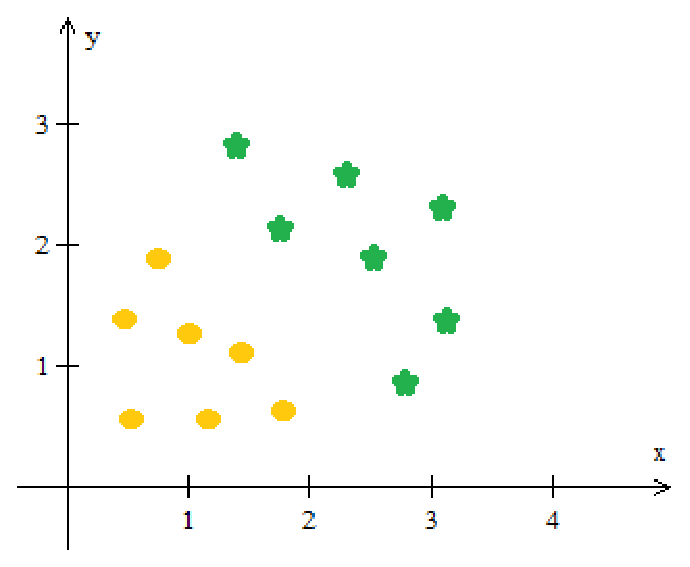
\includegraphics[scale=0.5]{graficos/linear_sepa}\label{fig1}}
\qquad
\subfigure[]{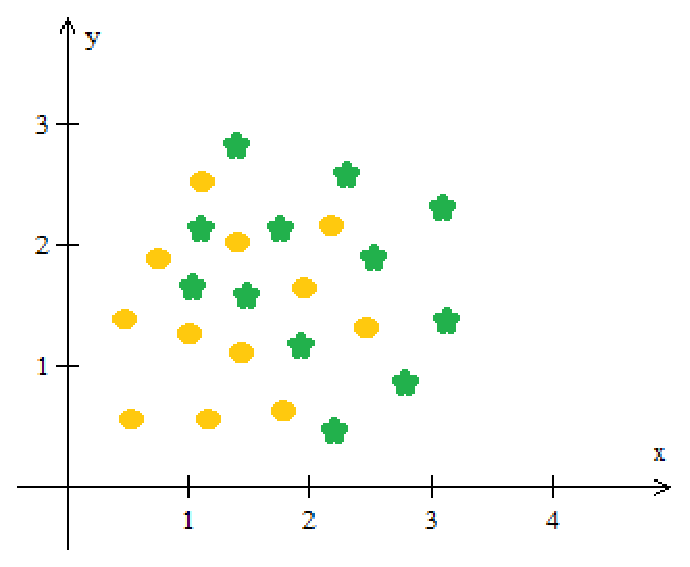
\includegraphics[scale=0.5]{graficos/linear_insepa}\label{fig2}}
\label{img:linear_sepa}
\caption{Em \ref{fig1} são apresentados dois conjuntos linearmente separáveis e em \ref{fig2} são apresentados dois conjuntos linearmente inseparáveis}
\end{figure}

É possível observar que na figura \ref{fig1} podem ser tratadas inúmeras retas seprando os dois conjuntos de pontos. Já na figura \ref{fig2} o modelo de programação linear poderá definir a melhor reta possível para separar os pontos.

A proposta do modelo e separa dois conjuntos de pontos, porém também pode ser utlizado em problemas onde busca-se a separação de múltiplos padrões. O presente trabalho foca nessa última abordagem, em todos os testes realizados o número de conjutnso de pontos é igual ou maior que três.

\section{O modelo}
Considerando dois conjuntos, no espaço n-dimensional $ R^{n} $, sendo o conjunto A representado pela matriz m x n, e o conjunto B representado pela matriz k x n. Contextualizando, k e m são as quantidades de pontos em cada conjunto, e n é a quantidade de características. O modelo gera um hiperplano que separa os pontos dos dois conjuntos. De forma que os m pontos do conjunto A fiquem de um lado do hiperplano e os k pontos do conjunto B fiquem do outro lado do hiperplano. Na figura abaixo o modelo é apresentado. E a seguir é apresentado de forma mais detalhada.

$$\min_{\omega ,\gamma ,y,z}\frac{e^{T}y}{m}+\frac{e^{T}z}{k}$$
$$s.a.\left\{\begin{matrix}-A\omega +e\gamma+e\leq y\\B\omega -e\gamma+e\leq  z\\ y\geq 0,y\geq 0\end{matrix}\right.$$

O modelo determina o hiperplano:
$$ x\omega = \gamma $$
Onde,  é $\omega$ o vetor normal ao hiperplano e $\gamma$ é um escalar. De forma que:
$$A\omega \geq e\gamma$$
e
$$B\omega \leq e\gamma$$
Onde e é um vetor de 1’s com dimensão m para o conjunto A e k para o conjunto B.
Para conjuntos linearmente separáveis torna-se fácil traçar um hiperplano separador, porém para conjuntos linearmente inseparáveis é necessária uma estratégia para que o hiperplano separador seja ótimo.
O modelo busca o melhor hiperplano, para isso gera dois hiperplanos limites somando 1 unidade a equação do hiperplano separador:
$$A\omega \geq e\gamma + e$$
e
$$B\omega \leq e\gamma - e$$
De forma que o hiperplano separador fica localizado exatamente entre esses dois hiperplanos limites.
Detalhando o modelo de acordo com \citeonline{Eberson10LPseparaPontos}, considerando x como um vetor em $ R^{n} $, definimos:

$1.\ \ (x_{i})_{+} = \max_{i=1,2,...,n}{\left \{x_{i},0  \right \}}$

$2.\ \ \left \| xx \right \|_{1} = \sum_{i=1}^{n}\left | x_{i} \right |$

Podemos escrever o problema de minimização com norma da seguinte forma:

$$\min_{\omega ,\gamma }\frac{1}{m}\left \| \left ( -A\omega + e\gamma  + e \right )_{+} \right \|_{1} + \frac{1}{k}\left \| \left ( B\omega - e\gamma + e  \right )_{+} \right \|_{1}$$

Seja $g:R^{n} \mapsto R^{m} , h:R^{n} \mapsto R^{k}$ e S um subconjunto de $R^{n}$ . Os problemas abaixo possuem soluções idênticas:

$$\min_{x\in S}\left \| g(x)_{+} \right \|_{1} + \left \| h(x)_{+} \right \|_{1}$$


$$\min_{x\in S} e^{t}y + e^{t}z\\$$
$$ s.a.\left\{\begin{matrix}y\geq g(x)\\ z\geq h(x)\\ y\geq 0, z\geq0\end{matrix}\right.$$

Como $g(x)_{+}\geq g(x)$ e $h(x)_{+}\geq h(x)$ podemos observar que os valores ótimos de y e z podem der dados pelas igualdades $y=g(x)_{+}$ e $z=h(x)_{+}$.

A partir do problema de minimização temos o problema de programação linear equivalente:

$\min_{\omega ,\gamma ,y,z}\frac{e^{T}y}{m}+\frac{e^{T}z}{k} \; \; \; \; (a)\\
s.a.\left\{\begin{matrix}-A\omega +e\gamma+e\leq y\; \; (b)\\B\omega -e\gamma+e\leq  z\; \; (c)\\ y\geq 0,y\geq 0\; \; (d)\end{matrix}\right.$

\underline{Dados do Modelo}:
\begin{itemize}
\item{m}: quantidade de imagens no conjunto correspondente a primeira expressão facial;
\item{k}: quantidade de imagens no conjunto correspondente a segunda expressão facial;
\item{A}: Matriz contendo o conjunto de vetores de caraterísticas das imagens correspondentes à primeira expressão facial;
\item{B}: Matriz contendo o conjunto de vetores de caraterísticas das imagens correspondentes à segunda expressão facial;
\item{e}:  vetor coluna unitário;
\end{itemize}

\underline{Variáveis do Modelo}:
\begin{itemize}
\item{$\omega$}: coeficientes do hiperplano que separa os conjuntos de imagens em dois grupos;
\item{$\gamma$}: constante do hiperplano que separa os conjuntos de imagens em dois grupos;
\item{y}: vetor contendo as distâncias de cada imagem do conjunto A ao hiperplano separador mais um;
\item{z}: vetor contendo as distâncias de cada imagem do conjunto B ao hiperplano separador mais um.
\end{itemize}

\underline{Formulação Matemática}:

	A função objetivo (a) procura minimizar a somas das médias das distâncias das imagens de ambos conjuntos. A restrição (b) exige que os pontos se encontrem necessariamente abaixo do hiperplano separador mais uma constante unitária.  A restrição (c) é análoga a restrição (b) aplicada as imagens da segunda expressão facial. As equações em (d) definem a natureza das variáveis do modelo, como sendo não negativas.

\section{Exemplo Ilustrativo do Modelo Classificador}
Para ilustrar o modelo vamos considerar dois exemplos em $R^{2}$ \cite{Bennett92robustlinear} de forma que a ilustração gráfica fique mais facilmente compreensível.
\begin{itemize}
\item Exemplo1:

Considerando as matrizes a seguir:
$$A=\begin{bmatrix}1 & 1\\ 1 & 2\\ 1 & 3\\ 2 & 1\\ 2 & 2\\ 2 & 3\\ 2 & 4\\ 3 & 3\\ 3 & 4\end{bmatrix}
B=\begin{bmatrix}4 & 1\\ 4 & 2\\ 4 & 3\\ 5 & 2\\ 5 & 3\\ 5 & 4\\ 6 & 2\end{bmatrix}$$

Nesse caso, temos: m = 9 (quantidade de pontos da matriz A) e k = 7 (quantidade de pontos da matriz B).  Submetendo as matrizes ao modelo temos:
\begin{itemize}
\item[$\ast$] Valor da função objetivo = 0
\item[$\ast$] $\omega$ = [-2  0]
\item[$\ast$] $\gamma$ = -7
\item[$\ast$] y = [0 0 0 0 0 0 0 0 0]
\item[$\ast$] z = [0 0 0 0 0 0 0]
\end{itemize}
Como o valor da função objetivo depende dos vetores y e z, podemos notar que o valor 0 indica que os conjuntos A e B são linearmente separáveis. A seguir é apresentada a representação gráfica dos pontos e das retas geradas pelo modelo.

\begin{center}
	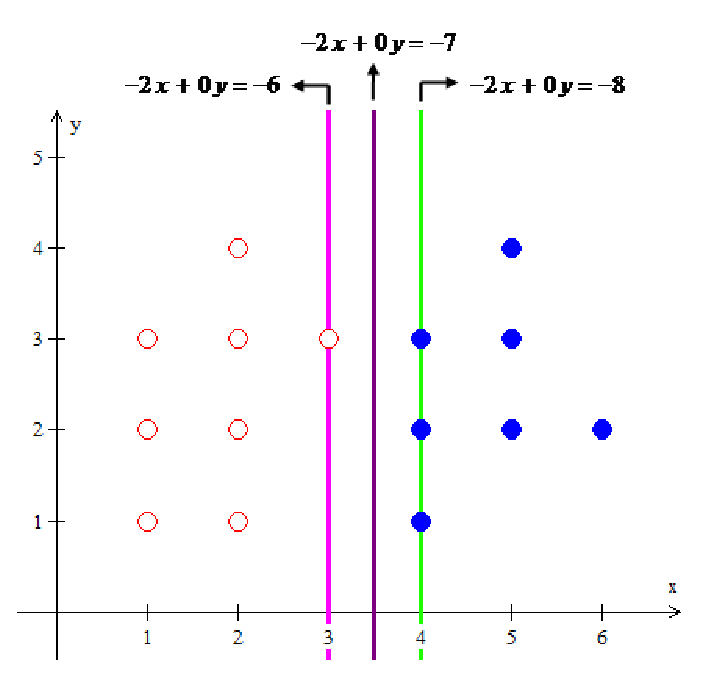
\includegraphics[scale=0.5]{graficos/exemplo2}
	\captionof{figure}{Representação ilustrativa do exemplo 1}
	\label{img:ex1}
\end{center}

A partir da representação gráfica podemos perceber que a reta separadora $-2x + 0y = -7$ se localizou exatamente no meio entre os dois conjuntos com o auxílio das duas retas: $-2x + 0y = -6$ e $-2x + 0y = -8$.

\item Exemplo2:
Vamos  considerar agora as matrizes:
$$A=\begin{bmatrix}3 & 4\\ 4.3 & 4.5\\ 4.5 & 2\\ 3 & 5.5\end{bmatrix}
B=\begin{bmatrix}4 & 2\\ 4.5 & 3.5\\ 5 & 3\end{bmatrix}$$

Neste exemplo temos: m = 4 e k = 3. De acordo com o modelo, temos os seguintes valores:
\begin{itemize}
\item[$\ast$] Valor da função objetivo = 0.92
\item[$\ast$] $\omega$ = [-0.91  0.91]
\item[$\ast$] $\gamma$ = -0.82
\item[$\ast$] y = [0 0 2.46 0]
\item[$\ast$] z = [0 0.91 0]
\end{itemize}

Com o valor da função objetivo diferente de zero, temos dois conjuntos linearmente inseparáveis, como ilustrado na figura a seguir.

\begin{center}
	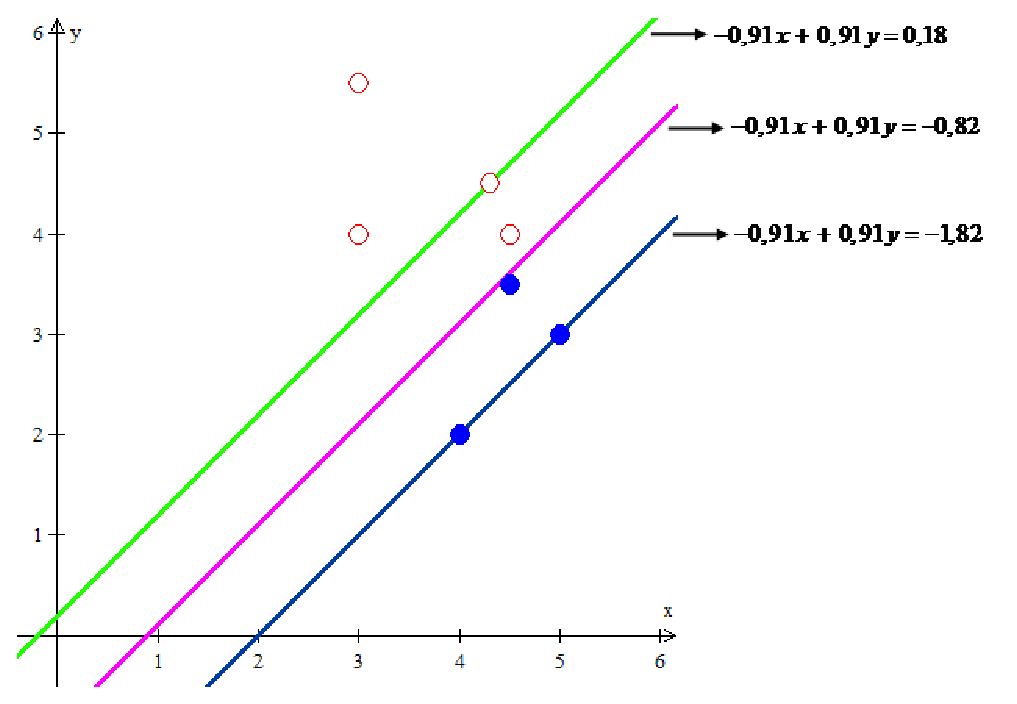
\includegraphics[scale=0.5]{graficos/exemplo1}
	\captionof{figure}{Representação ilustrativa do exemplo 2}
	\label{img:ex2}
\end{center}

Nesse exemplo notamos que o valor 2.46 no vetor y é referente ao ponto do conjunto A que está localizado do lado errado da reta. E o valor 0.91é referente ao ponto do conjunto B que está localizado mais próximo à reta separadora, apesar do ponto estar localizado do ponto correto da reta ele está localizado acima da reta limite $-0.91x + 0.91y = -1.82$.
\end{itemize}

\section{Etapa de classificação}
Após a geração dos classificadores utlizando o modelo de programação linear, é necessário um segundo procedimento onde ocorra de fato classificação de um vetor com padrão inicialmente desconhecido. Nessa etapa de classificação foi implementada uma estrutura de árvore de torneio.
Em seus trabalhos \citeonline{Feng} e \citeonline{Guo} utilizaram a estrutura de árvore de torneio na etapa de classificação após a utilização do modelo de programação linear para gerar os classificadores.
A seguir são apresentadas duas figuras para ilustrar o mecanismo da árvore de torneio.

\begin{center}
	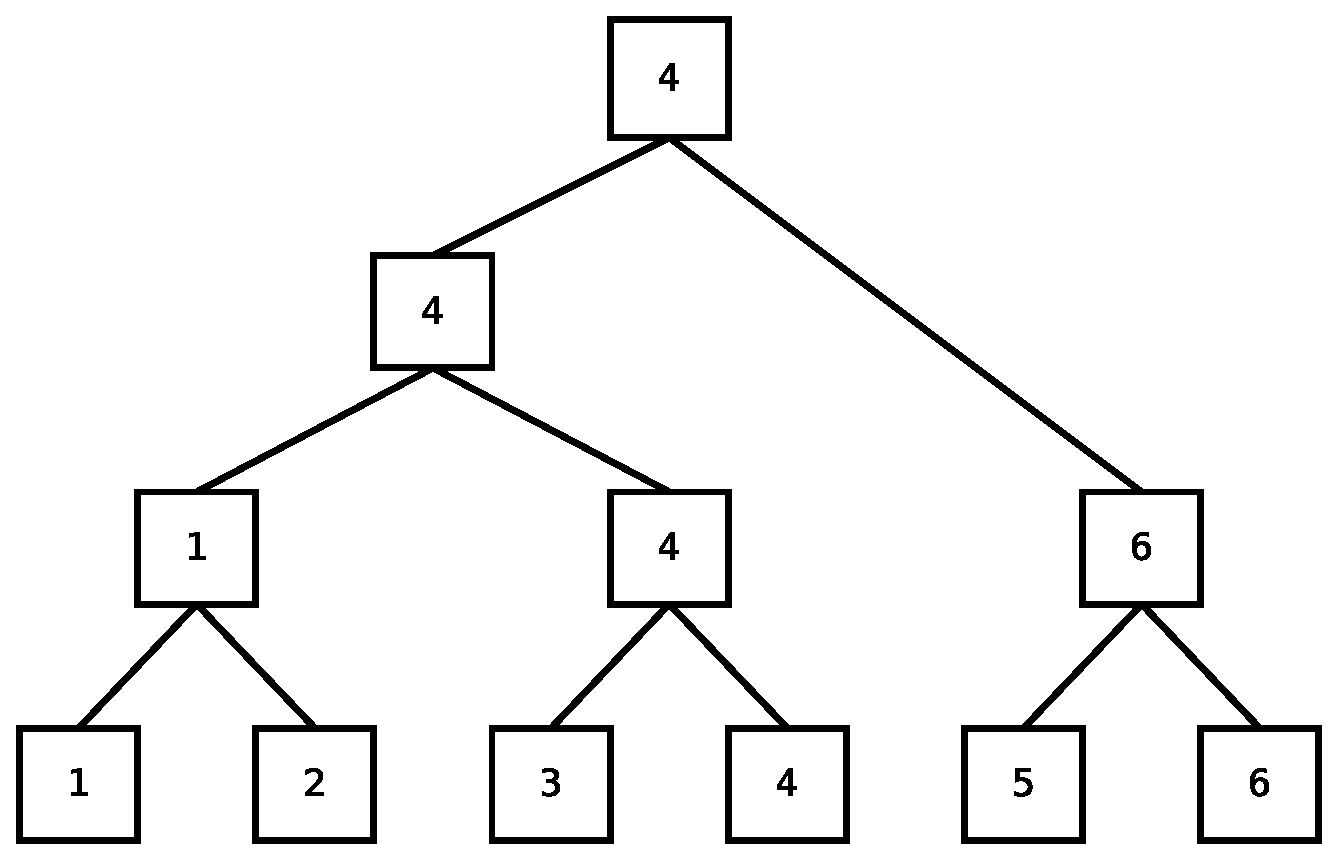
\includegraphics[scale=0.4]{graficos/ArvTorneio1}
	\captionof{figure}{Ilustração de uma árvore de torneio com 6 padrões}
	\label{img:ArvTorneio1}
\end{center}

\begin{center}
	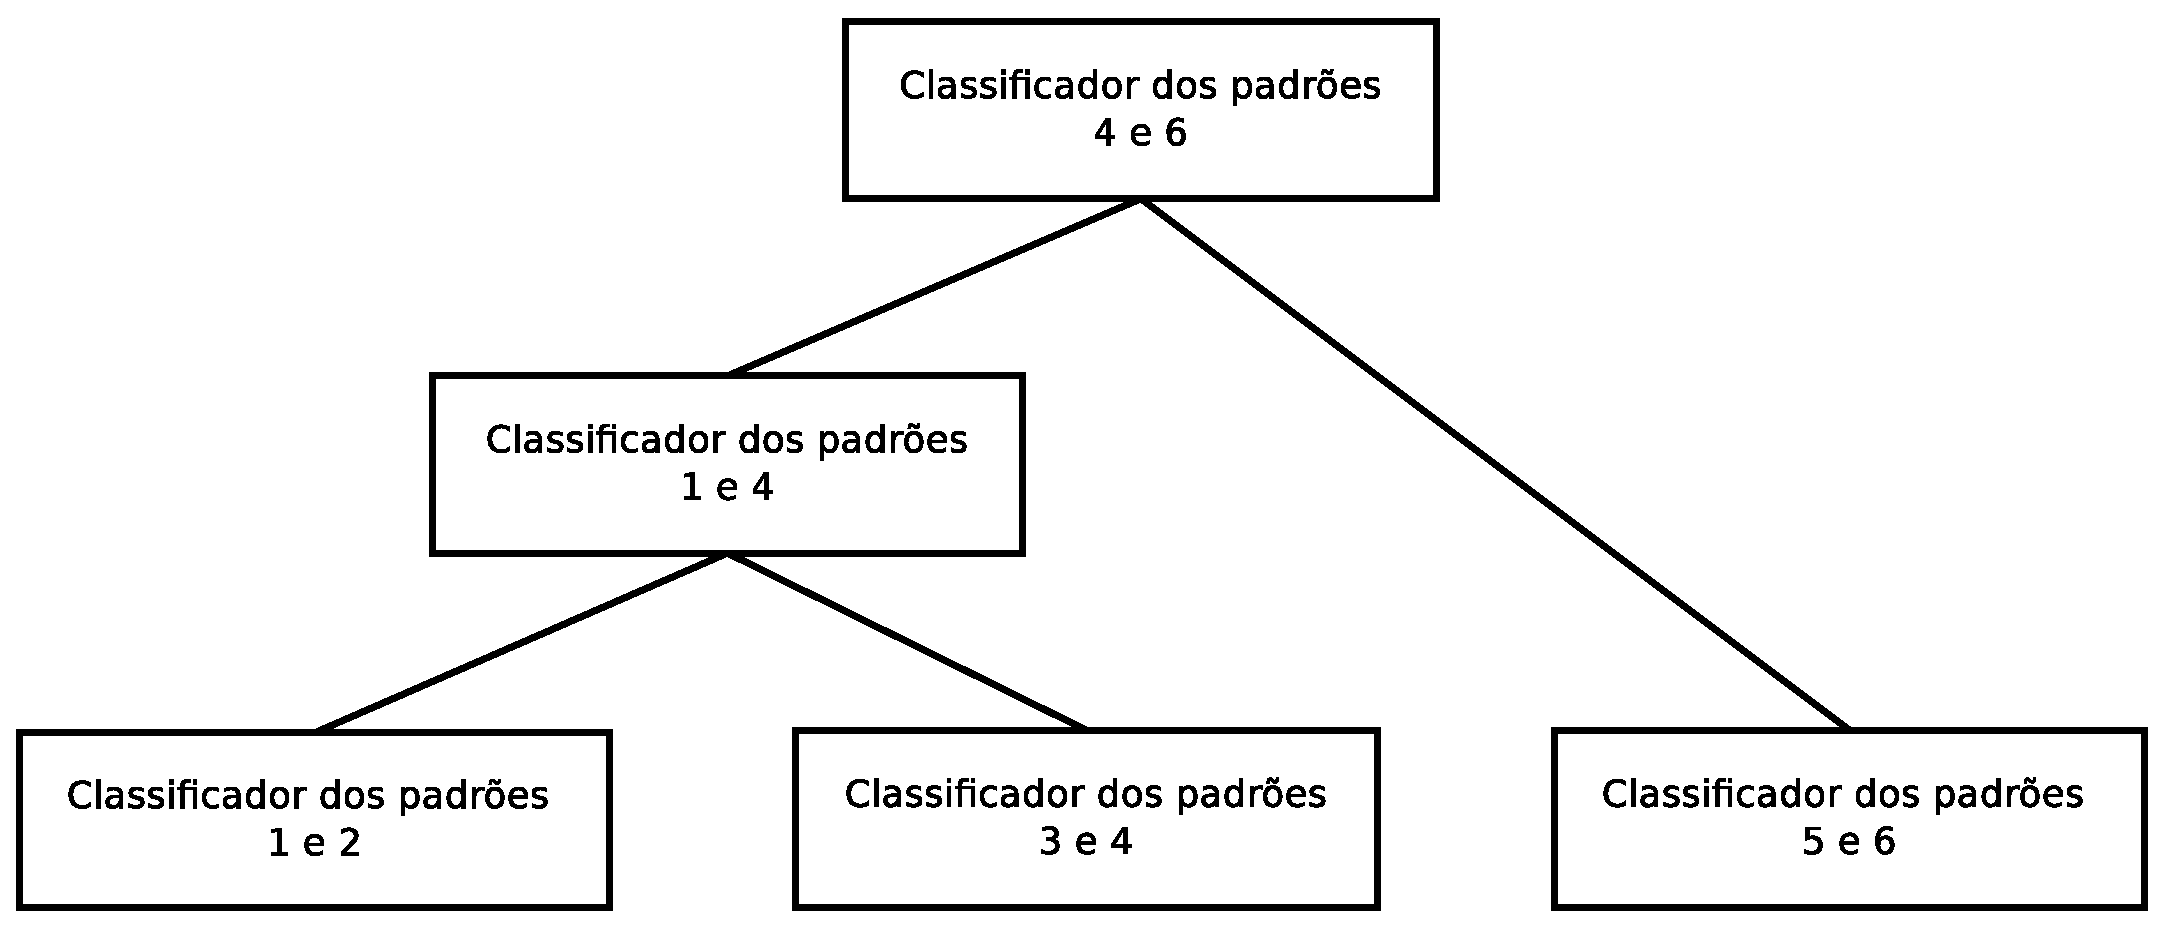
\includegraphics[scale=0.4]{graficos/ArvTorneio2}
	\captionof{figure}{Ilustração de uma árvore de torneio de acordo com os classificadores}
	\label{img:ArvTorneio2}
\end{center}
Depois de obtidos os hiperplanos separadores, é necessário um mecanismo para que um dado com padrão desconhecido possa ser classificado como um dos padrões, ou seja, analisando um vetor é preciso descobrir qual dos padrões ele se classifica. Para isso, é utilizada uma estrutura chamada árvore de torneio \cite{Feng} \cite{Guo}. Por analogia podemos pensar na árvore como a estrutura utilizada em um torneio esportivo e nos padrões como os times do torneio, os times devem se confrontar até que ao final saia o vencedor. Da mesma forma, analisamos os padrões até que ao final se obtenha o padrão ao qual o conjunto submetido pertença.
Na árvore da figura \ref{img:ArvTorneio1}, consideramos 6 padrões e o conjunto desconhecido pertencendo ao padrão 4. A quantidade de nós folhas deve ser a quantidade de padrões e a formação dos pares é arbitrária. Analisando o primeiro par, deve ser analisado em qual dos dois padrões o conjunto desconhecido mais se encaixa, ou seja, deve ser analisado de qual lado da reta (gerada pelo modelo quando foram submetidos os padrões 1 e 2, como ilustrado na figura \ref{img:ArvTorneio2})o conjunto desconhecido se encontra. Na figura exemplo, a maioria dos pontos ficaram localizados do mesmo lado da reta que os pontos do padrão 1, por isso esse padrão continuou no próximo nível da árvore e o padrão 2 foi excluído. Esse procedimento ocorre por analogia em todos os pares, até que ao final, quando analisados os padrões 4 e 6, foi definido que o vetor pertence ao padrão 4.

\chapter{Experimentos Computacionais}
Para a realização do experimentos computacionais foi necessário, primeiramente, obter os dados para teste e organizá-los para posteriormente submeter ao modelo para geração dos hiperplanos classificadores  e aos testes de classificação. Todos os experimento foram feitos utilizando um notebook com processador Intel Core i3, 2.27 GHz, 3 GB de RAM, sistema operacional Ubuntu 12.04, NetBeans IDE 7.1.2 e o software CPLEX da IBM.

Todo o processo, desde a organização dos dados até a etapa de classificação, foi implementado utilizando a linguagem de programação Java. A implementação foi feita em módulos, organizados da seguinte forma: Módulo organizador de dados, Módulo de geração de classificadores, Módulo de classificação, Módulo validador. No módulo organizador de dados os conjuntos de dados são organizados em subgrupos, cada subgrupo contendo vetores de todos os padrões, essa organização é importante para a etapa de validação do método. No Módulo de geração de classificadores está implementado o modelo de programação linear e são gerados os hiperplanos separadores. Os Módulos de classificação e validador são utilizados na etapa de teste, o primeiro realiza a classificação de um vetor em um dos padrões separados pelo hiperplano e o segundo realiza a validação do método de reconhecimento de padrões utilizando o método cross validation.

Na figura \ref{img:diagrama_modulos} estão representadas as principais etapas realizadas durante os experimentos computacionais.

\begin{center}
	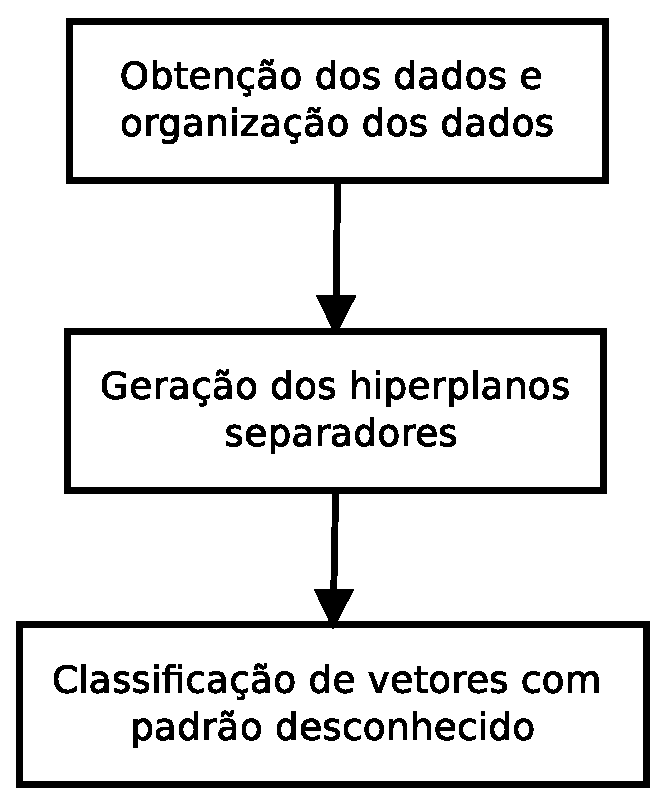
\includegraphics[scale=0.5]{graficos/diagrama_modulos}
	\captionof{figure}{Diagrama simples das etapas realizadas nos experimentos}
	\label{img:diagrama_modulos}
\end{center}

Primeiramente os dados foram obtidos já no formato de vetores de características ou extraídos de imagens, e depois foram divididos em subgrupos. Em seguida foram submetidos ao modelo de Programação Linear, responsável por gerar os classificadores e por último vetores com padrão desconhecido foram classificados. As duas últimas etapas são repetidas a cada ciclo de teste, essas repetições são controladas pelo Módulo validador. Nas seções seguintes essas etapas serão apresentadas de forma mais detalhada.

\section{Conjuntos de Dados}
Foram realizados testes com quatro conjuntos de dados: dígitos de 0 a 9 escritos manualmente, gestos da Língua Brasileira de Sinais, espécies da planta Iris e expressões faciais . Desses conjuntos, os três primeiros foram obtidos do repositório de dados \citeonline{Repositorio2013} e já estavam representados na forma de vetores de características. O último conjunto foi gerado a partir do conjunto de imagens JAFFE \cite{Jaffe}. A seguir são apresentadas as caraterísticas de cada um dos quatro conjuntos de dados:

\begin{itemize}
\item \textbf{Dígitos de 0 a 9 escritos manualmente \cite{Digitos}}
Na formação desse conjunto de dados 250 dígitos entre 0 e 9 foram escritos de forma aleatória por 44 pessoas, totalizando 11000 dígitos, porém estão disponíveis 10992 dígitos. Durante a coleta dos dados foram recolhidas, em intervalos fixos de 100 milissegundos, as coordenadas e a pressão da caneta sobre a superfície enquanto o dígito era escrito. No conjunto de dados utilizada foram considerados apenas os valores das coordenadas. Os dados foram reorganizados utilizando interpolação linear, foram utilizados 8 pontos, e obtidos vetores com 16 características.
Cada vetor é composto por 16 atributos que variam entre 0 e 100 e mais um valor variando entre 0 e 9 que representa o classe a qual o vetor pertence.
Os dados estão distribuídos como na tabela a seguir:
\begin{center}
	\begin{tabular}{cc}
        \hline
        Classe & Quantidade de instâncias \\
        \hline
		0 & 1143 \\
		1 & 1143 \\
		2 & 1144 \\
		3 & 1055 \\
		4 & 1144 \\
		5 & 1055 \\
		6 & 1056 \\
		7 & 1142 \\
		8 & 1055 \\
		9 & 1055 \\
        \hline
	\end{tabular}
	\label{tab:tabela_digitos}
        \captionof{table}{Quantidade de instâncias de cada dígito}
\end{center}

\item\textbf{Gestos da Língua Brasileira de Sinais (LIBRAS) \cite{Libras}}
Esse conjunto de dados é composta por 15 classes, ou seja, nela estão presentes 15 sinais da LIBRAS, sendo 24 instâncias de cada classe, totalizando 360 vetores de características. Os dados foram extraídos de vídeos com tempo médio de 7 segundos, em cada vídeo um movimento é executado e depois é representado como uma curva bidimensional. No pre processamento foram selecionados 45 frames de cada vídeo, em cada frame a coordenada do ponto central da mão é encontrado, compondo uma curva com 45 pontos. As coordenadas dos 45 pontos formam o vetor de características com 90 valores, os 45 primeiros valores representam o valor de x e o restante o valor de y.
O vetor de características tem no total 91 valores, sendo que 90 deles caracterizam o movimento e o último valor representa o padrão ao qual o vetor pertence.

\item \textbf{Espécies da planta Iris \cite{Iris}}
Nesse conjunto de dados são representados três tipos da planta Iris, é composta por 50 instâncias de cada tipo, totalizando 150 vetores. Cada vetor é composto por 4 características: comprimento da sépala, largura da sépala, comprimento da pétala, largura da pétala; e mais o nome da classe que o vetor representa.

\item \textbf{Expressões faciais}
No caso das expressões faciais, as imagens foram obtidas do conjunto de dados JAFFE \cite{Jaffe} e o pre processamento e a extração e características foram implementaos na linguagem de programação Python.
Inicialmente a proposta do presente trabalho era focar apenas na classificação de expressões faciais utilizando a programação linear. Durante a pesquisa não foi encontrada nenhum conjunto de dados que disponibilizasse os vetores de características da imagens, portanto foi necessária a implementação para a obtenção dos dados. Posteriormente foi verificado que seria necessário um aprofundamento do estudo na área da visão computacional, para que os vetores de caracteríticas não comprometessem o método classificador. Portanto esses dados foram obtidos através de uma implementação superficial de extração de caracteríticas.
Após a obtenção do banco de imagens JAFFE. As imagens foram recortadas a fim de isolar a região da face, utilizando linguagem de programação python, como mostrado na figura

\begin{center}
	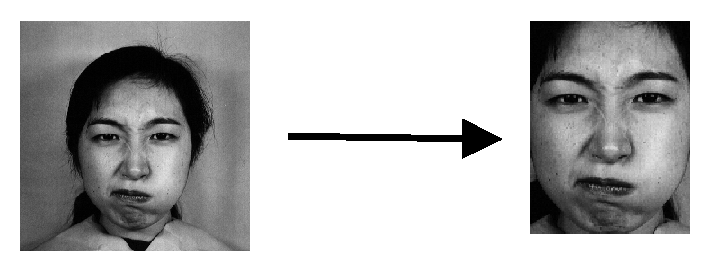
\includegraphics[scale=0.5]{graficos/jaffe}
	\captionof{figure}{Pre processamento das imagens do banco JAFFE}
	\label{img:jaffe}
\end{center}

O banco de imagens JAFFE é composto por 213 imagens, sendo divididas em 7 expressões: tristeza, alegria, desgosto, surpresa, raiva, medo e neutro. Na tebela \ref{tab:tabela_expressoes} é apresentada a quantidade de imagens para cada expressão.

\begin{center}
	\begin{tabular}{cc}
        \hline
        Classe & Quantidade de imagens \\
        \hline
		Tristeza & 31 \\
		Alegria & 31 \\
		Desgosto & 29 \\
		Surpresa & 30 \\
		Raiva & 30 \\
		Medo & 32 \\
		Neutro & 30 \\
        \hline
	\end{tabular}
	\captionof{table}{Quantidade de imagens para cada expressão}
        \label{tab:tabela_expressoes}
\end{center}

Na extração dos vetores de características foi utilizado o método Local Binary Patterns (LBP) que é um classificador de texturas. A cada pixel da imagem é atribuído um código, que é gerado a partir dos pixels ao redor. Tomando como referência o pixel central, a cada pixel vizinho é atribuído o valor 0 ou 1: se o valor do pixel vizinho for menor que o valor do pixel central, o valor 0 é atribuído, se for menor, o valor atribuído é 1. A partir daí, é gerado um código binário que é transformado em um valor decimal, esse valor decimal é o código LBP do pixel central \cite{LBPShan2009}. A figura abaixo demonstra como é calculado o código LBP.

\begin{center}
	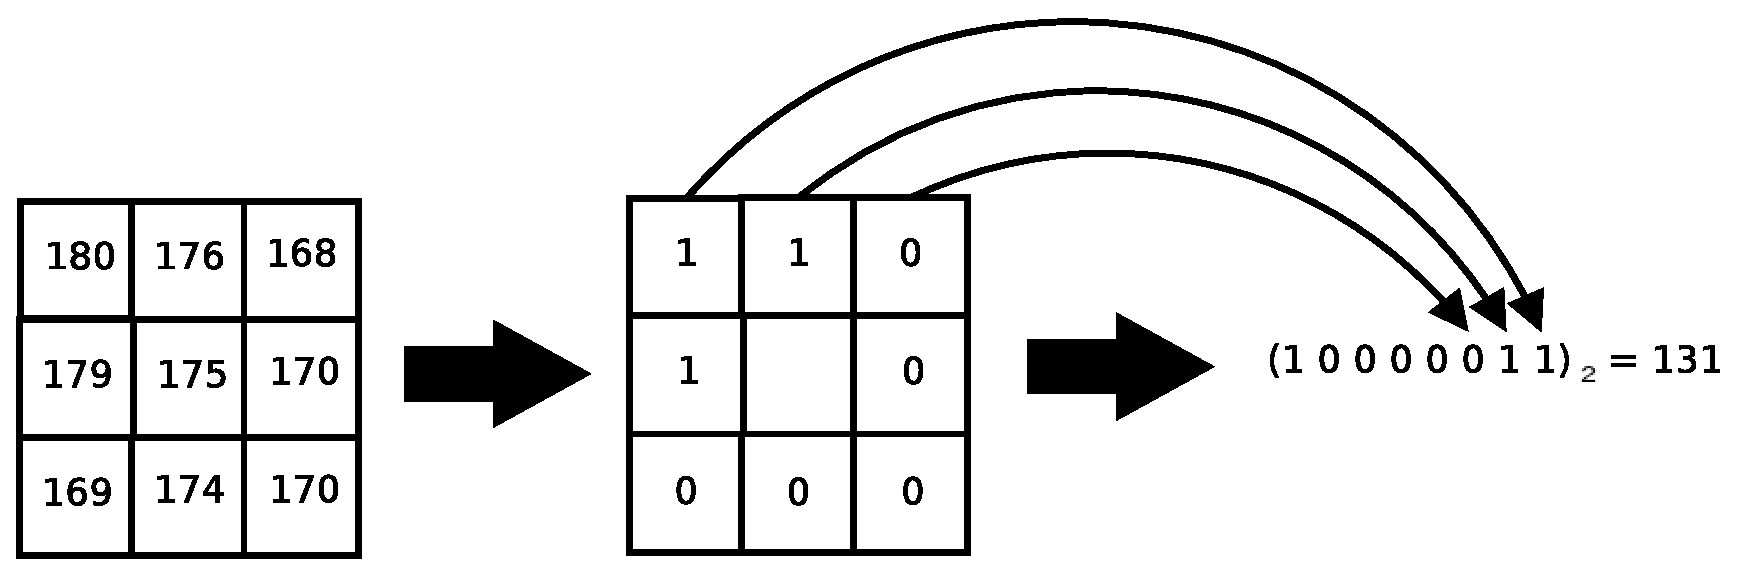
\includegraphics[scale=0.5]{graficos/LBP}
	\captionof{figure}{Cálculo do código LBP}
	\label{img:LBP}
\end{center}

Na implementação, primeiramente, a imagem é dividida em blocos, é gerado o histograma dos códigos LBP de cada bloco, por fim, os histogramas são concatenados. Esse resultado final é o descritor de texturas da imagem. A figura \ref{img:LBPHistograma} representa esse processo.

\begin{center}
	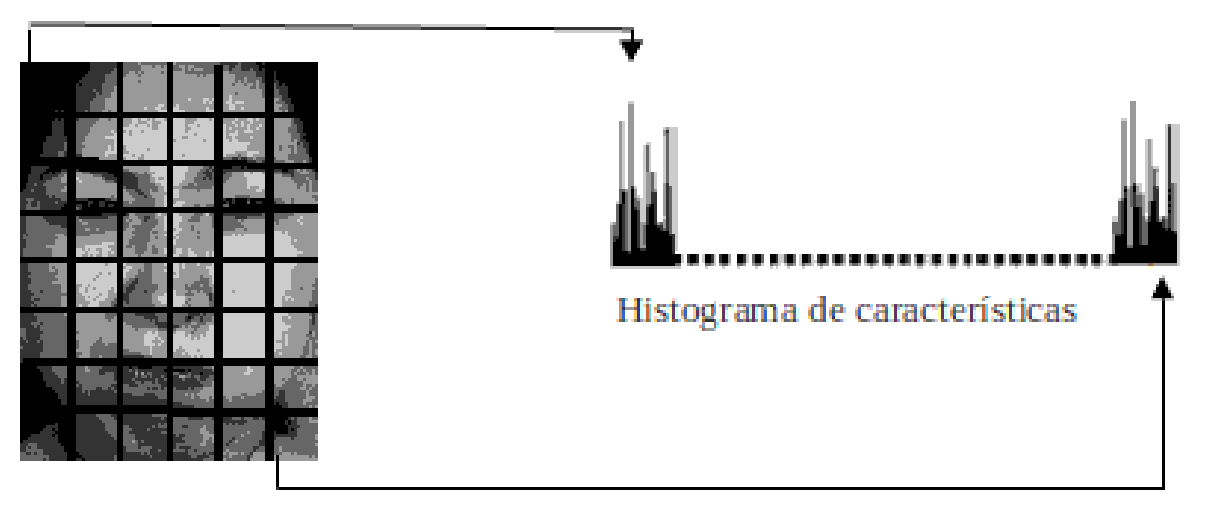
\includegraphics[scale=0.5]{graficos/histograma}
	\captionof{figure}{Representação da imagem dividida em blocos e da concatenação dos histogramas de cada bloco.}
	\label{img:LBPHistograma}
\end{center}

Para reduzir o tamanho do vetor de caracteríticas os códigos LBP de cada pixel são somados e divididos pelo número de imagens, qundo o resultado é menor do que um valor limiar os códigos desse pixel é excluído em todos os vetores \cite{Feng}. O limiar adotado nese caso foi 5 \cite{LBPShan2009}. Resultando em vetores de tamanho 843, sendo composto por 842 caracteríticas mais um dígito identificador do padrão. 
\end{itemize}

Nos vetores de características de todos os conjuntos de dados utlizados, é acrescido um valor informando a classe representada pelo vetor, para as etapas de treinamento e teste esse valor é omitido, ele só é utlizado na etapa de validação para verificar se o vetor foi corretamente classificado.

\section{Organização dos dados}
Em todos os testes foi o utilizado o método k -fold cross validation com k = 10, em seus trabalhos \citeonline{Baldisserotto05Validacao}, \citeonline{Kohavi95Cross}, \citeonline{Guo} utlizaram esse mesmo parâmetro. Os dados foram dividos em 10 subgrupos com mesmo tamanho \cite{Guo} e com a mesma quantidade de vetores para cada classe, por isso não foram em utlizados todos os dados de todos os conjuntos de dados.

\begin{center}
	\begin{tabular}{|p{2cm}|p{3cm}|p{2cm}|p{2cm}|}
        \hline
        \multicolumn{4}{|c|}{Conjuntos de dados} \\ \hline
        Nome & Total de vetores & Vetores utilizados & Quantidade de padrões\\ \hline
		Dígitos    &10992  & 10500 & 10\\ \hline
		LIBRAS     & 360   & 300   & 15\\ \hline
		Íris       & 150   & 150   & 3\\ \hline
		Expressões & 213   & 210   & 7\\ \hline
	\end{tabular}
        \captionof{table}{Organização dos dados}
	\label{table:org_dados}
\end{center}

Na tabela \ref{table:org_dados} constam informações dos quatro conjuntos de dados utlizadas como teste nomeadas da seguinte forma: Dígitos, LIBRAS, Íris, Expressões. Na segunda coluna são apresentados quantos vetores compõem o conjunto de dados no total sem distinguir o número de vetores por classe. E na última coluna são apresentados o número de vetores utlizados nos testes, em todos os casos o núemro de vetores utlizados é divisível por 10 por ser utlizado o parâmetro k = 10.

No conjunto de dados Dígitos, as classes que possuiam menos vetores eram as dos dígitos 3, 5, 8 e 9 com 1055 vetores, e as que possuiam mais vetores eram as dos dígitos 2 e 4 com 1144 vetores como mostrado na tabela \ref{tab:tabela_digitos}. Nessa caso, foram utilizados 1050 vetores de cada classe, totalizando 10500 vetores.

No conjunto de dados LIBRAS, cada classe possui 24 vetores, para a distribuição dos vetores entre os 10 subgrupos foram utlizados 20 vetores de cada classe, totalizando 300 vetores.

O conjunto de dados Íris possui 50 vetores para cada classe, possibilitando a utlização dos 150 vetores na distribuição entre os 10 subgrupos.

No quarto conjunto de dados, Expressões, a classe desgosto possui 29 vetores enquanto as classe restantes possuem 30 ou mais, como mostrado na tebela \ref{tab:tabela_expressoes}. Nesse caso, uma imagem da classe desgosoto foi repetida e utilizou-se 30 vetores para cada classe. 

Para esse conjunto de dados Expressões, se vetores fossem excluídos em todas as classes, o número de vetores divisível por 10, que é a quantidade de subgrupos, mais próximo é 20, o que acarretaria a exclusão de 9 ou mais imagens por classe, em contrapartida, na solução utlizada apenas 1 ou 2 imagens foram excluídas de cada classe, com exceção da classe desgosto que teve apenas uma imagem repetida. Já no conjunto de dados Dígitos optou-se pela exclusão, pois seria necessário repetir muitos vetores nas classes com o número mais baixo de vetores, o que poderia comprometer o resultado, o mesmo ocorre com o conjunto de dados LIBRAS.

\section{Resultados}
Nesta seção são apresentados os resultados encontrados nos testes realizados com os quatro conjuntos de dados anteriormento descritos. 

Na tabela a seguir são apresentados os resultados dos quatro conjuntos de dados após a validação 10-fold cross validation, a taxa de acerto é uma média das taxas obtidas em cada um dos 10 ciclos de teste. 

\begin{center}
	\begin{tabular}{|c|c|c|c|c|c|c|c|}
        \cline{1-7}
        \multicolumn{4}{ |c| }{Conjunto de dados} & \multicolumn{3}{ c| }{Vetores por padrão} \\
        \hline 
	Nome & Quantidade de   & Total de & Total & No          & Na & Taxa de\\ 
         ~   & características & vetores  &  ~    & treinamento & classificação & acerto (\%)
        \\  \hline
    	Dígitos    &        16     & 10500  & 1050 & 945   & 105 & 98\\ \hline
   	LIBRAS     &        90     &   300  &   20 &  18   &   2 & 72\\ \hline
    	Íris       &         4     &   150  &   50 &  45   &   5 & 87\\ \hline
    	Expressões &       842     &   210  &   30 &  27   &   3 & 34\\ \hline
	\end{tabular}
        \captionof{table}{Resultados após a validação 10-fold cross validation}
	\label{tab:resultados}
\end{center}

Na tabela \ref{tab:resultados} é aprsentada a quantidade de caracetrísticas presente em cada vetor de cada conjunto da dados, a quantidade de vetores de cada classe utilizados para treinamento e a quantidade de vetores de cada classe utilizados para teste a cada ciclo da validação cruzada. Na última coluna é apresentada a taxa média de classificações corretas ao final da validação.

Nessa tabela é possível observar que as classe com menos caracteríticas obtiveram as maiores taxas de acertos. Comparando os dois conjuntos com maioires taxas, observamos que o conjunto Dígitos com um número de vetores muito superior a do conjunto Íris obteve a maior taxa de acerto. O conjunto de dados Expressões, apesar de possuir uma quantidade de vetores superior a da classe LIBRAS, a quantidade de caracteríticas que é um número muito superior e possui a taxa de acerto mais baixa. 

Na tabela a seguir são apresentadas as taxas de acerto em cada ciclo de teste.

\begin{center}
	\begin{tabular}{|c|c|c|c|c|c|c|c|c|c|c|}
        \hline
        \multicolumn{1}{ |c| }{Conjunto} & \multicolumn{10}{ c| }{Taxas de acertos por ciclo de teste (\%)}
        \\ \cline{2-11}
	de dados  & C 1 & C 2 & C 3 & C 4 & C 5 & C 6 & C 7 & C 8 & C 9 & C 10 \\ \hline
    	Dígitos   & 0,98 & 0,98 & 0,98 & 0,98 & 0,98 & 0,98 & 0,98 & 0,97 & 0,96 & 0,97\\ \hline
   	LIBRAS    & 0,4  & 0,77 & 0,74 & 0,7 & 0,63 & 0,7  & 0,63 & 0,83  & 0,93 & 0,9 \\ \hline
    	Íris      & 0,74 & 0,8  & 0,93 & 0,87 & 0,93 & 0,74 & 0,87 & 0,87 & 0,93 & 0,87\\ \hline
    	Expressões& 0,34 & 0,38 & 0,38 & 0,33 & 0,29 & 0,29 & 0,24 & 0,43 & 0,33 & 0,43\\ \hline
	\end{tabular}
        \captionof{table}{Taxas de acerto em cada ciclo de teste}
	\label{tab:taxas}
\end{center}

Na tabela \ref{tab:taxas} pode ser observado que nos dados Dígitos houve menos variação na taxa. Nos dados Íris houve certa variação entre 74\% e 93\%. Os dados LIBRAS e Expressões, que são os que possuem os maiores vetores apresentaram uma maior varaiação. 

\subsection{Quantidade de vetores X Taxa de acerto}
Os conjuntos de dados são compostos por mais de um vetor de características de cada classe, e a quantidade de vetores pode influênciar na taxa de acertos final. Para fazer essa análise foi utilizado o banco de dados Dígitos por ser, entre os conjuntos utlizados, o que contém o maior número de vetores por classe.

\begin{center}
	 \begin{tabular}{|c|c|c|c|}
    \cline{1-3}
    \multicolumn{3}{|c|}{\textbf{Conjunto de dados Dígitos}}                     \\ \cline{1-3}
    \multicolumn{3}{|c|}{Vetores por padrão}                    \\ \hline
    Total                     & No treinamento & Na classificação & Taxa de \\ ~                         & ~              & ~                & acerto ( \% ) \\ \hline

    	   50   & 	45		   &		5	& 	0.898\\ \hline
   	  100   & 	90		   &	       10	&	0.926\\ \hline
	  200   &      180   		   &	       20	&	0.947\\ \hline
    	  300 	&      270		   &	       30	&	0.964\\ \hline
    	  500 	&      450  		   & 	       50	&	0.968\\ \hline
    	  600 	&      540		   &	       60	&	0.972\\ \hline
    	  900 	&      810		   &	       90	&	0.974\\ \hline
    	 1000 	&      900		   &	      100	&	0.975\\ \hline
    	 1050 	&      945		   &	      105	&	0.975\\ \hline
	\end{tabular}
        \captionof{table}{Quantidade de Vetores X Taxa de acerto}
	\label{tab:vetorxtaxa}
\end{center}

Na primeira coluna da tabela \ref{tab:vetorxtaxa} estão específicadas as quantidades de vetores de cada classe e nas duas colunas seguintes as quantidades de vetores de cada classe utilizados na etapa de treinamento e na etapa de testes respectivamente. Na útlima coluna estão específicadas as taxas de acertos em cada teste. 

É possível observar um aumento na taxa de acertos a medida que a quantidade de vetores cresce. Porém esse aumento não é proporcional ao aumento do núemro de vetores. A variação na taxa de acerto diminui a medida que a quantidade de vetores aumenta, do teste com 50 vetores por calsse para o teste com 100, houve uma variação de 2,8\% na taxa de acerto. Já no testes com 200 e 400 a variação na taxa foi de 2\%. E entre o teste com 600 vetores e o teste com quantidade máximamde vetores que é 1050 é observado uma variação bem pequena de 0,02\% na taxa de acerto.

\subsection{Tempo computacional}
A partir dos testes realizados também foram realizadas análises do ponto de vista computacional.
Os resultados mostrados na tabela a seguir são as médias dos tempos de 5 execuções incluindo a etapa de validação compĺeta, com os dez ciclos .

\begin{center}
\begin{tabular}{|c|c|c|c|c|c|}
\hline
\multicolumn{3}{ |c| }{Conjuntos de dados} & \multicolumn{3}{ c| }{Tempo de execução (em segundos)} \\ \hline
Nome       & Quantidade & Vetores & Gerador de  & Gerador de  & Treinamento  \\ 
  ~        &     de     &    por  & hiperplanos & hiperplanos &     e        \\
  ~        &  padrões   &  padrão & por ciclo   & total       & Classificação \\   \hline
Dígitos    &     10     &  1050   &   2,18      &   21,88     &    30,53 \\ \hline
Libras     &     15     &    20   &   0,65      &    6,47     &     7,87 \\ \hline
Iris       &      3     &    50   &   0,04      &    0,41     &     0,65 \\ \hline
Expressões &      7     &    30   &   0,78      &    7,82     &     8,93 \\ \hline


\end{tabular}
        \captionof{table}{Tempos computacionais}
	\label{tab:tempocomp}
\end{center}

Na terceira linha da tabela \ref{tab:tempocomp} estão os tempos de execução apenas do módulo de geração de classificadores, que é o módulo onde o modelo de programação linear é resolvido. É possível constatar um tempo computacional para a geração dos classificadores corresponde a mais de 50\% do tempo computacional total. A quantidade de classificadores gerados deve ser considerada. Na quinta coluna é apresentado o tempo médio para geração dos classificadores a cada ciclo de teste e na segunda linha da tabela são apresentadas as quantidades de classificadores gerados nesse tempo, para três conjuntos de dados esse tempo foi inferior a 1 segundo.

Na última linha da tebla \ref{tab:tempocomp} são apresentados os tempos totais de execução de cada experimento. Pode-se constatar que esse tempo é proporcional ao tamanho dos vetores do conjunto de dados e a quantidade de classes. O conjunto de dados Íris obteve um tempo computacional menor que 1 segundo sendo um conjunto de dados com 3 classe e 50 vetores para cada classe. Enquanto o conjunto de dados Dígitos obteve o maior tempo computacional apesar de possuir vetores com 16 caracteríticas é o conjunto de dados com maior número de vetores por classe. 

Comparando os tempos computacionais dos conjuntos Dígitos e Expressões é possível verificar que a quantidade de vetores por classe teve maior influência no tempo de execução, já que a diferença dos tempos de execução das duas classes é bastante alto, proporcional a diferença entre as quantidades de vetores por classe. 

A mesma observação pode ser feita comparando os tempos dos conjuntos LIBRAS e Expressões, ainda que o número de classe do conjunto LIBRAS seja mais que o dobro do número de classes do conjunto Expressões, cada vetor do conjunto Expressões possui muitas características a mais que os vetores do conjunto LIBRAS e o tempo computacional do conjunto Expressões foi superior ao tempo do conjunto LIBRAS.

\section{Análise dos Resultados}

Juntamente com o conjunto de dados Dígitos \cite{Digitos}, estão disponíveis resultados de testes utilizando como metódo de classificação K nearest neighbor, a métrica utlizada para medir as distâncias entro os K vizinhos mais próximos foi a distância Euclidiana. O autor testou variando o parâmetro K de 1 à 11 com a taxa de acerto variando entre 97,34\% e 97,80\%. Em relação ao experimentos realizados neste trabalho é possível verificar que utilizando o método proposto foram obtidas taxas de acertos próximas as encontradas em \citeonline{Digitos}.

Em seu trabalho \citeonline{Swan2012Iris} abordou a classificação de padrões utlizando Redes Neurais e o conjunto de dados Íris. O autor dividiu 75 vetores para treinamento e 75 para teste. Foram realizados 3 testes, variando um parâmetro na configuração da rede neural. As taxas de acertos obtidas variaram entre 83,33\% e 96,66\%. No experimento utilizando o modelo de programação linear a media de acertos obtida foi de 87\%, um taxa que supera a obtida utilizando redes neurais, dependeno da configuração.

Em \citeonline{Feng} foi utilizado o conjunto de dados JAFFE \cite{Jaffe}. O modelo de programação linear proposto em \citeonline{Bennett92robustlinear} é utlizado para gerar os classificadores e na classificação de imagens com expressão desconhecida foi utilizada uma árvore de torneio, assim como nos experimentos deste trabalho. A taxa de acerto foi de 93.8\%.

No trabalho de \citeonline{Guo} também foi utilizado o banco JAFFE \cite{Jaffe}. Foram feitas comparações entre aluns métodos de classificação, entre eles: Bayes com taxa de acertos 71,0\%, Support Vector Machine linear e não linear, com taxa de acertos 92,4\% e 91,9\%, respectivamente e uma variação do modelo de programação linear utilizado neste trabalho, com taxa 91,0\%. Em todos os casos foram utilizados mecanismos para seleção das características que seriam utlizadas
 
Tanto no trabalho de \citeonline{Feng} quanto no trabalho de \citeonline{Guo} foram obtidas taxas consideravelmente mais altas do que a obtida nos experimentos (34,0\%). Essa diferença pode ser atribuída pela falta de pre processamento das imagens, como já comentado anteriormente.


\chapter{Conclusão}

A programação linear, apesar de possuir aplicações em diversas áreas, não é tão explorada na área da computação. O presente trabalho aprsentou a utilização de uma modelo de programação lienar na separação de padrões. Como resultado, esse modelo gera hiperplanos separadores que são utlizados na tarefa de classificar um dado com padrão inicialmente desconhecido. E todos os experimentos realizados o número de padrões é igual ou amior que três.

Inicialmente foi realizado um estudo sobre modelos e plaicações de programação linear e sobre métodos de resolução, princiaplmente sobre o meodo simplex revisado, um método desenvolvido para problemas de programação linear resolvidos computacionalmente. Também foram aprsentados alguns metódos de classificação de padrões de validação de modelos.

Foram realizados experimentos utilizando quatro bases de dados, três dessas bases foram obtidas já no formato de vetores de carcaterísticas. No caso da base de dados Expressões, foram obtidas imagens e os vetores de características foram extraídos utilizando o método Local Binary Patterns. Nos experimentos, o modelo de programação linear proposto por \citeonline{Bennett92robustlinear} foi utlizado, os padrões foram combinados em pares e os vetores de cada padrão submetidos ao modelos, gerando um hiperplano separador para cada combinação. Já na etapa de classificação foi utlizada uma estrtura de árvore binária de torneio, o vetor a ser classificado era subemtido a árvore e um padrão era retornado classificando esse vetor. Para a validação do modelo o método k -fold cross valdiation foi utlizado devido a variação de tamanho das bases de dados utilizadas. Na implementação foi utlizada a linguagem de programação JAVA e o software CPLEX da IBM.

Nos experimentos foram obtidos resultados EXCELENTES??? para os casos da base de dados Dígitos e Íris, com taxas de acerto 98\% e 87\%, respectivamente. No caso da base de dados LIBRAS foi obtida uma taxa de acertos de 74\%. Para a base de dados Expressões a taxa obtida foi de 34\%, esse resultado pode ser atribuído ao vetor de caracteríticas, já que os vetores foram extraídos sem um pre processamento das imagens. Utlizando a base de dados Dígitos foi analisada a influência da quantidade de dados na melhoria da taxe de acertos, foi verificado que essa taxa pode aumentar a medida que a quantidade de dados por padrão aumenta, porém após uma certa quantidade de vetores por classe, o aumento na taxa de acerto não é tão significante. Já no teste para análise do tempo computacional foi constatado que a quantidade de padrões e de vetores por padrões influencia no tempo, porém a quantidade de vetores tem uma maior influencia no aumento do tempo computacional.

O presente trabalho expôs uma aplicação na programação linear na computação, mais especificamente na classificação de padrões. Essas aplicações contribuem na interação mais transparente homem - máquina.
Foram obtidos bons resultados em alguns experimentos, e em alguns casos, superiores ao resultados obtidos em outros trabalhos que utilizaram a mesma base de dados e um método de classificação diferente. Em outros experimentos os resultados obtidos  não foram tão satisfatórios.

Como trabalho futuro propõe-se a melhoria na taxa de acertos, principalmente da base de dados Expressões. Para isso deve haver um estudo amis aprofundado na área da visão computacional, submetendo as imagens a um pre processamento e utilizando uma método mais apurado para selecionar as características e reduzir o tamanho do vetor de características.

Um outra melhoria é o tempo computacional, que poderia ocorrer através de um estudo sobre as melhores estrturas de dados a serem utlizadas.   

%--------------------------------- Bibliografia --------------------------------

\citeoption{abnt-repeated-author-omit=yes}
\bibliographystyle{abnt-alf}
\bibliography{bibliografia}

\end{document}

